\documentclass[a4paper, 12pt]{article}

\usepackage{mathtext}
\usepackage[T2A]{fontenc}
\usepackage[utf8]{inputenc}
\usepackage[russian]{babel}

\usepackage{amsmath}
\usepackage{titlesec}
\usepackage{scrextend}
\usepackage{graphicx}
\usepackage{tikz}
\usetikzlibrary{shapes.misc}
\usepackage{pdflscape}
\usepackage{float}
\usepackage{pgfplots}

\DeclareSymbolFont{T2Aletters}{T2A}{cmr}{m}{it}
\graphicspath{ {./images/} }
\pgfplotsset{compat=newest}

% Установки для отрисовки решеток кодера
\tikzstyle{lightedge}=[dashed]
\tikzstyle{mainedge}=[solid]
\tikzstyle{activeedge}=[green, very thick]
\tikzstyle{inputBit}=[rectangle,fill=red, text=white]
\tikzstyle{outputBit}=[rectangle,fill=blue, text=white]
\tikzstyle{pointer}=[orange,->,dashed]
\tikzstyle{highlight}=[circle,fill=blue,text=white,scale=0.7]

\newcounter{ctra}
\newcommand{\trellisEdges}[2]{
  \setcounter{ctra}{#2}
  \pgfmathtruncatemacro{\xplusone}{#1 + 1}
  \ifodd\value{ctra}
      \draw[mainedge] (s#1#2) -- (s\xplusone2);
  \else
      \draw[mainedge] (s#1#2) -- (s\xplusone0);
  \fi
  \ifodd\value{ctra}
      \draw[lightedge] (s#1#2) -- (s\xplusone3);
  \else
      \draw[lightedge] (s#1#2) -- (s\xplusone1);
  \fi
}

% #1=x; #2=y; #3=In; #4=Out
\newcommand{\trellisInOut}[4]{
  \node[inputBit] (in#1) at (#1+0.5,4) {#3};
  \node[outputBit] (out#1) at (#1+0.5,5) {#4};
  \draw[pointer] (in#1) -- (#1+0.5,#2);
}

% #1=x; #2=y; #3=In
\newcommand{\trellisIn}[2]{
  \node[outputBit] (in#1) at (#1+0.5,4) {#2};
}


\author{Анатолий Копыл}
\title{Расчёт основных характеристик цифровой системы связи с использованием квадратурной модуляции}

\begin{document}

% НАЧАЛО ТИТУЛЬНОГО ЛИСТА
\makeatletter
\begin{titlepage}
  \begin{center}
    \hfill \break
    \footnotesize{ФЕДЕРАЛЬНОЕ ГОСУДАРСТВЕННОЕ БЮДЖЕТНОЕ ОБРАЗОВАТЕЛЬНОЕ УЧРЕЖДЕНИЕ}\\ 
    \footnotesize{ВЫСШЕГО ПРОФЕССИОНАЛЬНОГО ОБРАЗОВАНИЯ}\\
    \small{\textbf{«Санкт-Петербургский государственный университет телекоммуникаций им. проф. М. А. Бонч-Бруевича»}}\\
    \hfill \break
    \normalsize{Факультет инфокоммуникационных сетей и систем}\\
    \hfill \break
    \normalsize{Кафедра теоретических основ связи и радиотехники}\\
    \hfill\break
    \hfill \break
    \hfill \break
    \hfill \break
    \large{ \@title }\\
    \hfill \break
    \hfill \break
    \normalsize{Учебная дисциплина <<Теория электрической связи>>}\\
    \hfill \break
    \hfill \break
    \hfill \break
    \normalsize{Курсовая работа}\\
    \hfill \break
    \hfill \break
  \end{center}
    
  \hfill \break
  \hfill \break
  
  \normalsize{
    \hfill\begin{minipage}{\dimexpr\textwidth-6cm}
      Студент группы ИКТО-91 Копыл А. В.\\
      зачетная книжка № 1905141\\\\
      Руководитель \underline{\hspace{4cm}}
    \end{minipage}
  }\\
  \vfill
  \begin{center} Санкт-Петербург 2021 \end{center}
  \thispagestyle{empty} % выключаем отображение номера для этой страницы
\end{titlepage}
\makeatother
% КОНЕЦ ТИТУЛЬНОГО ЛИСТА
  
\newpage

Цель курсовой работы -- изучить и разработать систему цифровой связи, 
оптимальную в отношении флуктуационной помехи и исключающую появления 
межсимвольной помехи.

\section{Структурная схема системы\\цифровой связи}

Система связи предназначена для передачи аналоговых сообщений
по цифровому каналу связи.
\begin{figure}[H]
  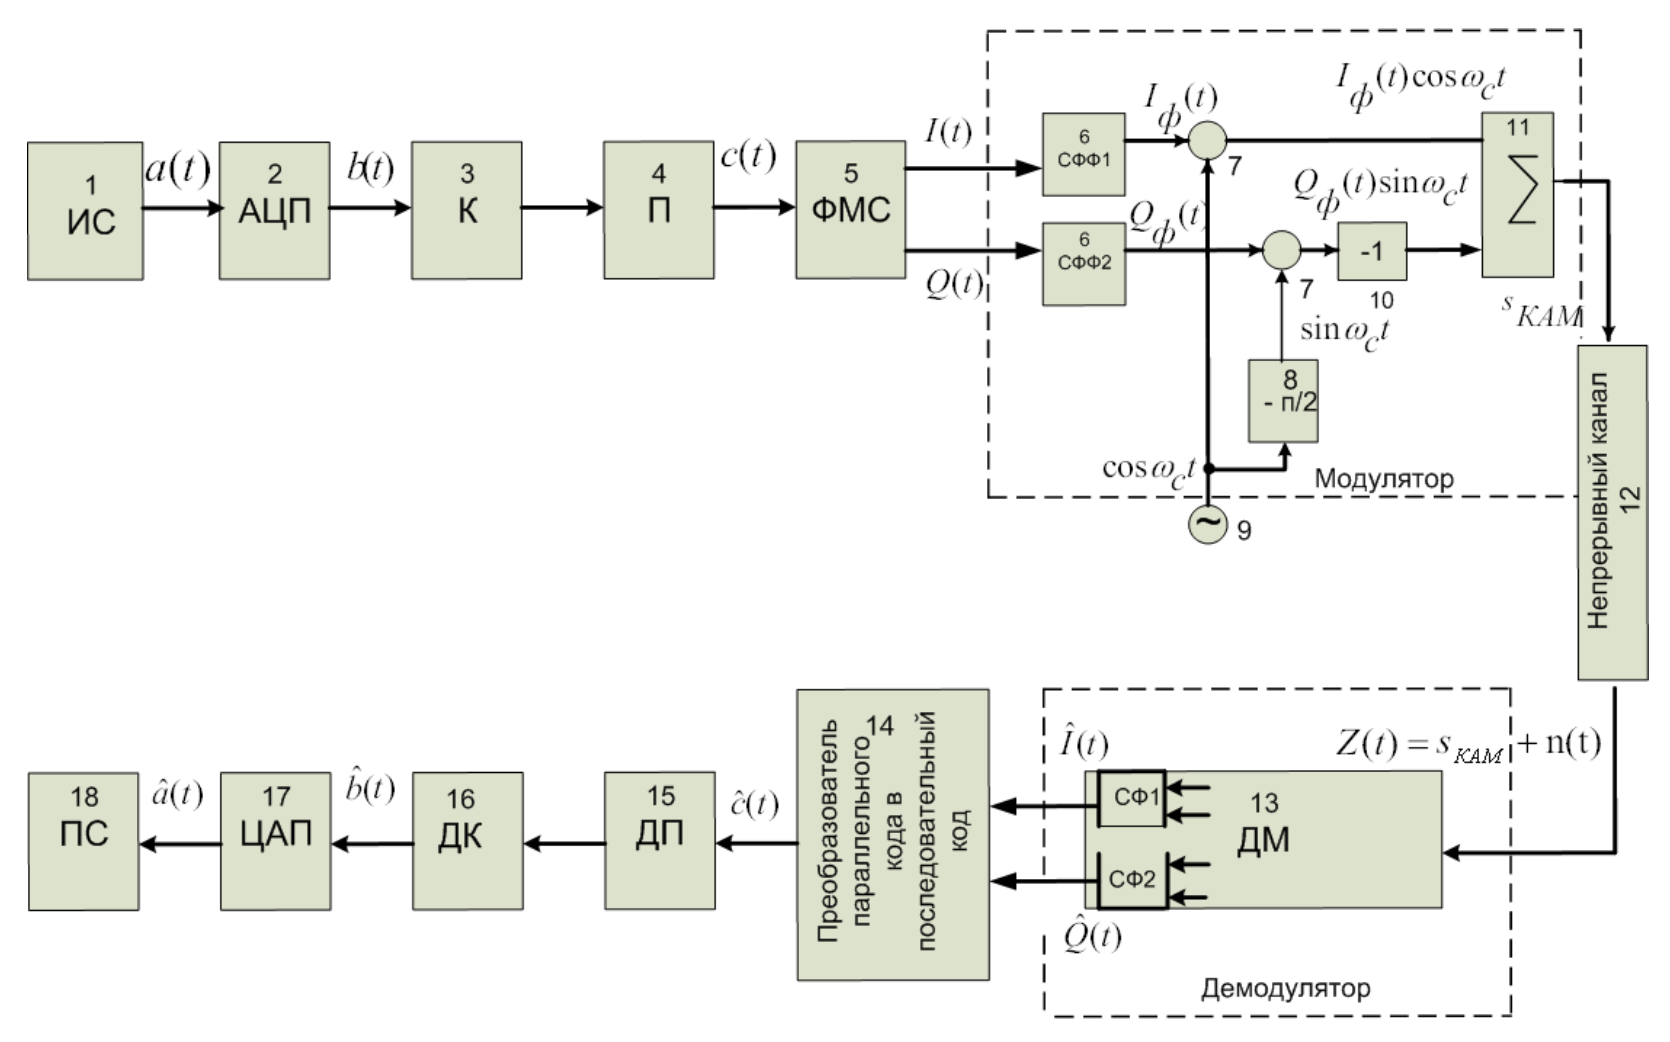
\includegraphics[scale=0.5]{struct_scheme}
  \caption{Структурная схема цифровой системы связи}
  \label{fig:struct_scheme}
\end{figure}

В систему входят следующие функциональные узлы с последующими назначениями:
\begin{enumerate}
  \item Источник сообщений -- создает реализации $a(t)$ случайного
  процесса $A(t)$.
  \item Аналого-цифровой преобразователь -- преобразует аналоговый
  сигнал от источника сообщения в последовательность 
  двоичных отсчетов $b(t)$.
  \item Кодер -- включает в цифровой поток от АЦП дополнительные
  символы, предназначенные для повышения помехоустойчивости системы
  связи;
  \item Формирователь модулирующих символов -- служит для получения
  модулирующих сигналов $I(t)$ и $Q(t)$, соответствующих заданному
  виду модуляции;
  \item Сглаживающие формирующие фильтры (СФФ1, СФФ2);
  \item Перемножители -- для получения БМ сигналов: синфазного 
  $I(t)\cos{\omega_Ct}$ и квадратурного $Q(t)\sin{\omega_Ct}$.
  \item Фазовращатель -- для получения второго несущего колебания, 
  ортогонального по отношению к первому;
  \item Генератор гармонических колебаний -- для получения несущего  
  колебания;
  \item Инвертор;
  \item Сумматор -- для объединения синфазного и квадратурного 
  сигналов в единый сигнал с квадратурной модуляцией 
  $S_{КАМ}(t) = I(t)\cos{\omega_Ct} + Q(t)\sin{\omega_Ct}$;
  \item Непрерывный канал -- среда распространения сигнала 
  $S_{КАМ}(t)$;
  \item Демодулятор -- для анализа приходящего сигнала, 
  искаженного помехами, и принятии решения о переданном сообщении; 
  \item Преобразователь параллельного кода в последовательный код --
  для преобразования сигнала с выхода демодулятора в 
  последовательный формат кодовых комбинаций;
  \item Декодер -- для исправления части ошибок, возникших при приёме 
  сообщения $\hat{b}(t)$ вследствие влияния помех; 
  \item Цифро-аналоговый преобразователь -- для восстановления  
  аналоговой формы сигнала $\hat{a}(t)$ из его цифрового представления;
  \item Получатель сообщений.
\end{enumerate}

\section{Исходные данные}
$m=41$
\begin{center}
  \begin{tabular}{ | p{5cm} | p{5cm} | p{5cm} | } 
    \hline
    Предельные уровни аналогового сигнала \(a_{мин}\), \(a_{макс}\) (В) & \(a_{макс}=25,6\) В;\newline\(a_{мин}=-25,6\) В & Внести свои данные \\
    \hline
    Верхняя частота спектра аналогового сигнала \(f_В\) & \(f_В =(1+m\cdot 10^{-2})\cdot 10^4\) & \(f_В =14100\) \\ 
    \hline
    Заданный уровень квантования & \(j=500-3\cdot m\) & 377 \\
    \hline
    Спектральная плотность мощности флуктуационной помехи & 41 & \(N_0=2,3\cdot 10^{-7}\, В^2/Гц\)\\
    \hline
    q -- номер тактового интервала ошибки & \(q=m\mod{3}+1\) & \(q=3\)\\
    \hline
    Вид модуляции & КАМ-16 & \\
    \hline
  \end{tabular}
\end{center}

\section{Расчет составляющих системы цифровой связи}

\subsection{Источник сообщений}
Источник сообщения (ИС) вырабатывает реализации $a(t)$ стационарного
случайного процесса $A(t)$, типа квазибелого шума с параметрами 
$a_{мин}$, $a_{макс}$ и $f_В$. Мгновенные значения сообщения
равновероятны в интервале от значения $a_{мин}$ и до значения 
$a_{макс}$.

Требуется:
\begin{enumerate}
  \item Написать аналитические выражения для плотности вероятности 
  $w(а)$ мгновенных значений сообщения, функции распределения $F(a)$ и
  построить их графики (рис. \ref{fig:prob_plots}).

  \[ w(a)=\frac{1}{a_{макс}-a_{мин}}=\frac1\Delta=\frac{1}{25,6+25,6}=0,02 \]
  \[ F(a)=\int^a_{-\infty}w(a)da=
  \int^a_{a_{мин}}\frac{1}{\Delta}da=
  \begin{cases}
    1, & a > a_{макс}\\
    \frac{a-a_{мин}}{\Delta}, & a_{мин} \leq a \leq a_{макс}\\
    0, & a < a_{мин}
  \end{cases}\]
  где $\Delta = a_{макс}-a_{мин}=51,2\, В$.

  % Графики
  \begin{figure}[H]
    \centering
    \begin{tikzpicture}
      \pgfmathsetmacro{\amin}{-25.6}
      \pgfmathsetmacro{\amax}{25.6}
      \begin{axis}[
        width=6cm,height=4cm,
        axis lines = left,
        xlabel = $a$,
        ylabel = {$F(a)$},
        xmin=-40, xmax=40,
        ymin=0, ymax=1.25,
      ]
        \addplot [
          domain=-40:\amin, 
          color=red,
        ]
        {0};
        \addplot [
          domain=\amin:\amax,
          samples=2,
          color=red,
        ]
        {(x-\amin) / 51.2};
        \addplot [
          domain=\amax:40, 
          color=red,
        ]
        {1};
      \end{axis}
    \end{tikzpicture}%
    \begin{tikzpicture}
      \pgfmathsetmacro{\amin}{-25.6}
      \pgfmathsetmacro{\amax}{25.6}
      \begin{axis}[
        width=6cm,height=4cm,
        axis lines = left,
        xlabel = $a$,
        ylabel = {$w(a)$},
        xmin=-40, xmax=40,
        ymin=0, ymax=0.03,
      ]
        \addplot [
          domain=-40:\amin, 
          color=blue,
        ]
        {0};
        \addplot [
          domain=\amin:\amax,
          samples=2,
          color=blue,
        ]
        {0.02};
        \addplot [
          domain=\amax:40, 
          color=blue,
        ]
        {0};
        \draw [dashed] (axis cs:\amin,0) -- (axis cs:\amin,0.02);
        \draw [dashed] (axis cs:\amax,0) -- (axis cs:\amax,0.02);
      \end{axis}
    \end{tikzpicture}
    \caption{Графики функции распределения и плотности вероятности}
    \label{fig:prob_plots}
  \end{figure}
  \item Рассчитать математическое ожидание $\overline{A(t)}$ и 
  дисперсию $D\{A(t)\}$ сообщения $A(t)$.
  \[ \overline{A(t)}=\int^\infty_{-\infty}a\cdot w(a)da=
  \int^{a_{макс}}_{a_{мин}}a \frac{1}{a_{макс}-a_{мин}} da=
  \frac{a^2}{2\Delta} \Biggr|^{a_{макс}}_{a_{мин}}\! =
  \frac{a_{макс}^2-a_{мин}^2}{2\Delta}=0 \]

  \begin{align*}\begin{split}
    D\{A(t)\}&=\int^\infty_{-\infty}(a-\overline{A(t)})^2 w(a)da=
    \int^{a_{макс}}_{a_{мин}}a^2w(a)da\\
    &=\frac{a^3}{3\Delta}\Biggr|^{a_{макс}}_{a_{мин}}\!
    =\frac{a_\text{min}^2+a_\text{max}a_\text{min}+a_\text{max}^2}{3}
    =218,5
  \end{split}\end{align*}
  \item Написать аналитическое выражение для спектральной плотности
  мощности $G_A(f)$ сообщения $A(t)$ и построить график 
  (рис. \ref{fig:spectr_plot}).
  \[ G_A(f)=\frac{D\{A(t)\}}{2f_В}=\frac{218,5}{2\cdot1,41\cdot 10^4}
  =7,7 \,мВ^2/Гц \]
  \[ G_A(f)=\begin{cases}
    7,7 \,мВ^2/Гц, & |f| \leq f_B\\
    0, & |f| > f_B
  \end{cases} \]
  \begin{figure}[H]
    \centering
    \begin{tikzpicture}
      \pgfmathsetmacro{\fv}{14100}
      \pgfmathsetmacro{\Gaf}{0.0077}
      \begin{axis}[
        width=6cm,height=4cm,
        axis lines = left,
        ylabel = {$G_A(f)$},
        xmin=-\fv*1.5, xmax=\fv*1.5,
        ymin=0, ymax=\Gaf*1.5,
      ]
        \addplot [
          domain=-\fv*1.5:-\fv, 
          color=blue,
        ]
        {0};
        \addplot [
          domain=-\fv:\fv,
          samples=2,
          color=blue,
        ]
        {\Gaf};
        \addplot [
          domain=\fv:\fv*1.5, 
          color=blue,
        ]
        {0};
        \draw [dashed] (axis cs:-\fv,0) -- (axis cs:-\fv,\Gaf);
        \draw [dashed] (axis cs:\fv,0) -- (axis cs:\fv,\Gaf);
      \end{axis}
    \end{tikzpicture}
    \caption{График спектральной плотности мощности}
    \label{fig:spectr_plot}
  \end{figure}
  \item Найти аналитическое выражение для корреляционной функции
  $B_A(\tau)$ сообщения $A(t)$ и построить график 
  (рис. \ref{fig:coorel_plot}). 
  По форме графика $B_A(\tau)$ определить, 
  является ли сообщение $A(t)$ эргодическим случайным процессом 
  или не является таковым.

  \begin{align*}\begin{split}
    B_A(\tau)&=\int^\infty_{-\infty}\frac{G_A(f)}{2}e^{j2\pi f\tau}df
    =\int^{f_B}_{-f_B}\frac{G_A}{2}\cos{2\pi f\tau}df\\
    &=\frac{G_A}2 \frac{\sin{2\pi f \tau}}{2\pi \tau}\Biggr|^{f_B}_{-f_B} 
    =G_A\frac{\sin{2\pi f_B \tau}}{2\pi\tau}
  \end{split}\end{align*}
  \begin{figure}[H]
    \centering
    \begin{tikzpicture}
      \pgfmathsetmacro{\PI}{3.14159}
      \pgfmathsetmacro{\fv}{14100}
      \pgfmathsetmacro{\Ga}{0.0077}
      \begin{axis}[
        width=10cm,height=6cm,
        axis lines = left,
        ylabel = {$B_A(\tau)$},
        xlabel = {$\tau$},
      ]
        \addplot [
          color=blue,
          samples=100,
          domain=-0.01:0.01,
        ]
        {\Ga*(sin(2*\PI*\fv*x))/(2*\PI*x)};
      \end{axis}
    \end{tikzpicture}
    \caption{График корреляционной функции $B_A(\tau)$}
    \label{fig:coorel_plot}
  \end{figure}
\end{enumerate}

\subsection{Аналого-цифровой преобразователь}
Аналого-цифровой преобразователь (АЦП) преобразует реализации 
аналогового (непрерывного) сообщения $A(t)$ в цифровую 
форму, в поток двоичных символов: нулей и единиц, 
т. е. в последовательность прямоугольных импульсов, 
где «0» имеет нулевое напряжение, а «1» -- прямоугольный 
импульс положительной полярности. 
Амплитуда импульсов $U$ равна 1 В.

Преобразование аналогового сигнала в цифровую форму 
осуществляется в три этапа.

На первом этапе производится дискретизация реализации 
$a(t)$ сообщения $A(t)$ по времени. В моменты времени $t_i$ 
берутся непрерывные по уровню отсчеты $a(t_i)$ 
мгновенных значений реализации $a(t)$. Расстояние
между отсчетами равно интервалу $\Delta t$, величина которого
определяется в соответствии с теоремой Котельникова:
\[\Delta t \leq \frac{1}{2f_B};\, 
f_d=\frac{1}{\Delta t}\geq2f_B\]
где $f_d$ -- частота дискретизации.

На втором этапе выполняется квантование точных отсчетов 
$a(t_i)$ по уровню. Для этого интервал $\Delta$, равный 
разности $\Delta=a_{макс} - a_{мин}$, разбивается на уровни 
квантования с постоянным шагом $\Delta a =0,1\, В$. 
Уровни квантования нумеруются целыми числами 
$0,1,2,3,...,L-1$. Нумерация уровней начинается с уровня, 
которому соответствует значение $a_мин$, и заканчивается на 
уровне, которому соответствует значение $a_макс$. Обычно
величина шага квантования $\Delta a$ выбирается так, чтобы 
число уровней квантования $L$ можно было представить в виде 
$L=2^k$, где $k$ -- целое число. 

Каждый аналоговый отсчет $a(t_i)$ заменяется значением 
ближайшего к нему уровня квантования $j$ в виде целого числа, 
удовлетворяющего неравенству $0\leq j \leq L-1$. 
Получаем квантованный отсчет $j_{10}(t_i)$ в виде целого 
числа в десятичной форме счисления.

На третьем этапе число $j_{10}(t_i)$ в десятичной форме 
переводится в двоичную форму счисления $j_2(t_i)$ в виде 
последовательности $k$ двоичных
символов и на выходе АЦП появляется сигнал в виде двоичной цифровой последовательности из $k$ информационных символов.

Требуется:
\begin{enumerate}
  \item Рассчитать интервал дискретизации $\Delta t$ для 
  получения непрерывных отсчетов $a(t_i)$ реализации 
  $a(t),\, t_i=i\cdot\Delta t,\, i=0,\pm1,\pm2,...$.
  \[ \Delta t \leq \frac{1}{2f_B}=\frac1 {2\cdot 14100} = 3,546\cdot 10^{-5}\, с \]
  \item Рассчитать частоту дискретизации $f_d$.
  \[ f_d=\frac{1}{\Delta t}\geq 2f_B=\frac{1}{3,546\cdot 10^{-5}}=28200 \]
  \item Определить число уровней квантования $L$.
  \[ k=9;\, L=2^9 = 512 \]
  \item Рассчитать мощность шума квантования $P_{ШК}$
  и сравнить ее с мощностью непрерывного сообщения $A(t)$.
  \[ P_{ШК}=\Delta a^2/12
  =\frac{0,1^2}{12}=8,33\cdot10^{-4}\, В^2 \]
  \[ P_{A(t)}=A^2(t)=1\, В^2\]
  \[ P_{A(t)} >> P_{ШК} \]
  \item Найти минимальное число $k$ двоичных разрядов, 
  требуемое для записи в двоичной форме любого номера $j$ 
  из $L-1$ номеров уровней квантования.
  \[ L-1=511_{10}=111111111_2 \]
  \[ k_{люб}=9 \]
  \item Записать $k$-разрядное двоичное число, 
  соответствующее заданному уровню квантования $j$.
  \[ j=377_{10}=101111001_2 \]
  \item Начертить временную диаграмму отклика АЦП 
  $b_{АЦП}(t)$ на заданный уровень квантования $j$ 
  в виде последовательности импульсов, 
  сопоставляя единичным символам прямоугольные импульсы 
  положительной полярности, а нулевым -- нулевые напряжения. 
  Амплитуда импульсов $U$ равна $2h$ B. Над импульсами 
  надписать значения соответствующих двоичных информационных 
  символов (ДИС). Длительность отклика АЦП на каждый отсчет 
  не должна превышать интервала дискретизации $\Delta t$.
  \begin{figure}[H]
    \centering
    \begin{tikzpicture}
      \draw[->, very thick] (0,1) -- (9.2,1);
      \draw[->, very thick] (0,-0.2) -- (0,2.2);

      \draw (0,2) -- (1,2) -- (1,0);
      \draw (1,0) -- (2,0) -- (2,2);
      \draw (2,2) -- (6,2) -- (6,0);
      \draw (6,0) -- (8,0) -- (8,2);
      \draw (8,2) -- (9,2);

      \node at (0.5,2.5) {$1$};
      \node at (1.5,2.5) {$0$};
      \node at (2.5,2.5) {$1$};
      \node at (3.5,2.5) {$1$};
      \node at (4.5,2.5) {$1$};
      \node at (5.5,2.5) {$1$};
      \node at (6.5,2.5) {$0$};
      \node at (7.5,2.5) {$0$};
      \node at (8.5,2.5) {$1$};
    \end{tikzpicture}
    \caption{Временная диаграмма отклика АЦП}
  \end{figure}
\end{enumerate}

\subsection{Кодер}
Используется помехоустойчивый сверточный код.

\begin{enumerate}
  \item Параметры сверточного кода.
  \begin{itemize}
    \item Степень кодирования $k/n=1/2$,
    \item длина кодового ограничения $K=3$,
    \item векторы связи $\overline g_1=111$ и 
    $\overline g_2=101$,
    \item импульсная характеристика $h(k)=111011000...$,
    \item кодовое расстояние $d=5$.
  \end{itemize}

  \item Структурная схема кодера.
  \begin{center}
    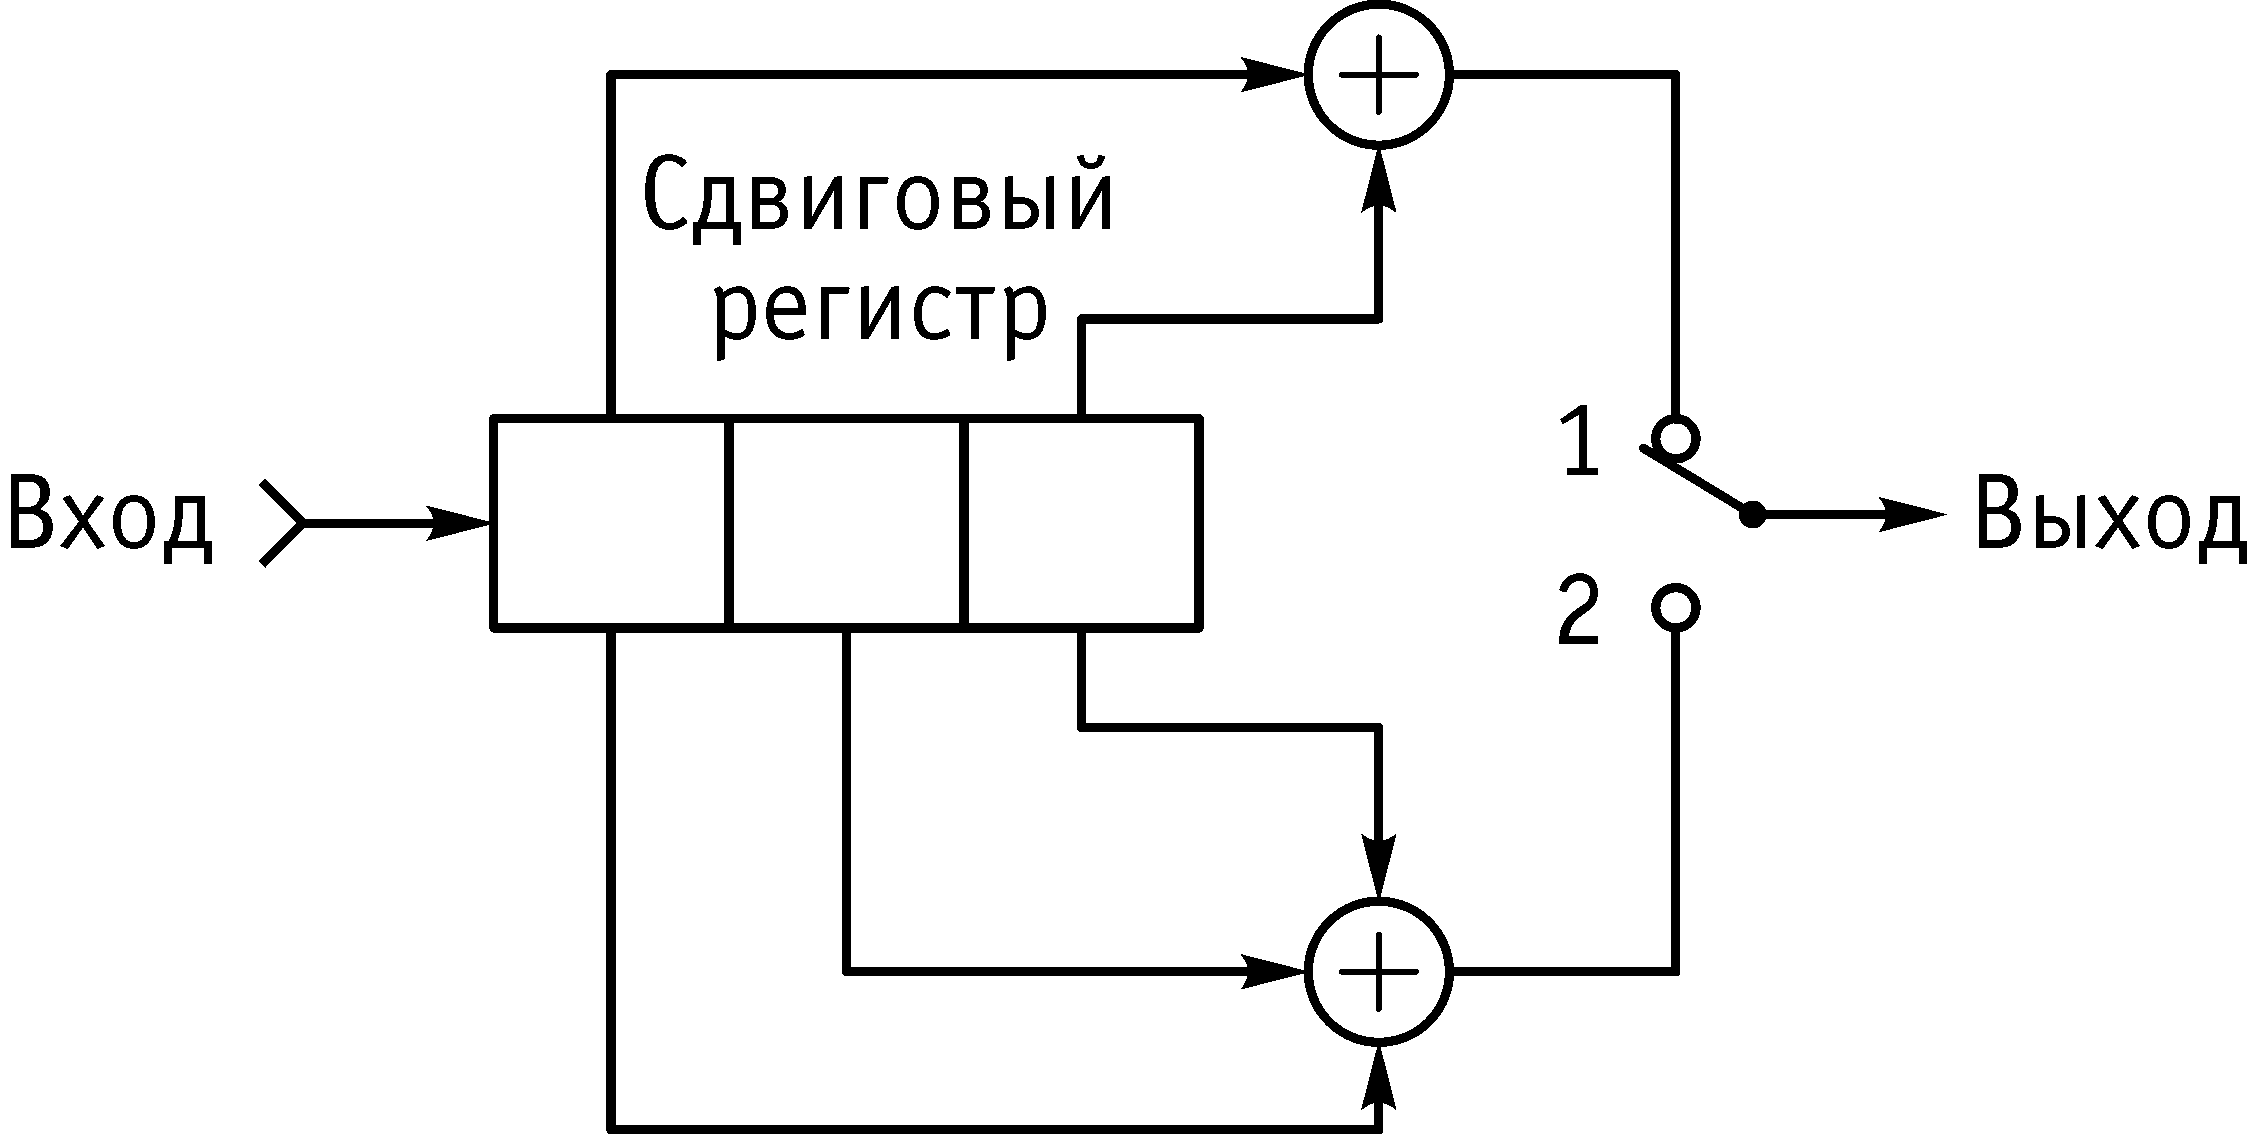
\includegraphics[scale=0.8]{coder2}
  \end{center}

  \item Решетчатая диаграмма кодера.
  \begin{figure}[H]
  \begin{tikzpicture}[x=1cm, y=-1cm]
    \node at (-0.5,0) [left] {$s_1=00$};
    \node at (-0.5,1) [left] {$s_2=10$};
    \node at (-0.5,2) [left] {$s_3=01$};
    \node at (-0.5,3) [left] {$s_4=11$};

    % Nodes
    \foreach \x in {0,...,12} {
      \node at (\x,-.7) {$\x$};
      \foreach \y in {0,...,3} {
        \node (s\x\y) at (\x,\y) [circle,fill=black,scale=0.7] {};
      }
    }

    % Edges
    \trellisEdges{0}{0}
    \trellisEdges{1}{0}
    \trellisEdges{1}{1}
    \foreach \x in {2,...,11} {
      \foreach \y in {0,...,3} {
        \trellisEdges{\x}{\y}
      }
    }
  \end{tikzpicture}

  \caption{Решетка кодера} \label{fig:coder_empty}
\end{figure}


  \item По решетчатой диаграмме сверточного кодера определить
  последовательность кодовых символов (КС) $\overline u$ на выходе кодера 
  при условии, когда на вход кодера поступает 9-разрядная 
  двоичная последовательность информационных символов (ИС) 
  $\overline m$, соответствующая заданному уровню квантования $j$.
  \begin{center}
    \begin{tabular}{ |c|c|c|c|c|c|c|c|c|c|c|c|c|c| }
      \hline
      ИС &1&0&1&1&1&1&0&0&1&0&0&0&0\\
      \hline
      КС &11&10&00&01&10&10&01&11&11&01&11&00&00\\
      \hline
    \end{tabular}
  \end{center}
  \[ \overline u = 11 10 00 01 10 10 01 11 11 01 11 00 00 \]

  \item На решетчатой диаграмме кодера отметить путь, 
  соответствующий полученным КС.
  \begin{figure}[H]
  \begin{tikzpicture}[x=1.2cm, y=-1cm]
    \node at (-0.5,0) [left] {$s_1=00$};
    \node at (-0.5,1) [left] {$s_2=10$};
    \node at (-0.5,2) [left] {$s_3=01$};
    \node at (-0.5,3) [left] {$s_4=11$};

    % Nodes
    \foreach \x in {0,...,9} {
      \node at (\x,-.7) {$\x$};
      \foreach \y in {0,...,3} {
        \node (s\x\y) at (\x,\y) [circle,fill=black,scale=0.7] {};
      }
    }

    % Edges
    \trellisEdges{0}{0}
    \trellisEdges{1}{0}
    \trellisEdges{1}{1}
    \foreach \x in {2,...,8} {
      \foreach \y in {0,...,3} {
        \trellisEdges{\x}{\y}
      }
    }

    % Inputs and Outputs
    \node at (-0.5,4) [left] {Входной бит};
    \node at (-0.5,5) [left] {Результат};

    \trellisInOut{0}{0.5}{1}{11}
    \trellisInOut{1}{1.5}{0}{10}
    \trellisInOut{2}{1.5}{1}{00}
    \trellisInOut{3}{2}{1}{01}
    \trellisInOut{4}{3}{1}{10}
    \trellisInOut{5}{3}{1}{10}
    \trellisInOut{6}{2.5}{0}{01}
    \trellisInOut{7}{1}{0}{11}
    \trellisInOut{8}{0.5}{1}{11}
  \end{tikzpicture}

  \caption{Решетка кодера} \label{fig:coder}
\end{figure}
\end{enumerate}

\subsection{Формирователь модулирующих символов}
Формирователь модулирующих символов служит для получения
модулирующих сигналов $I(t)$ и $Q(t)$, соответствующих заданному
виду модуляции.

Требуется:
\begin{enumerate}
  \item Изобразить сигнальное созвездие для заданного вида модуляции.
  \begin{figure}[H]
    \centering
    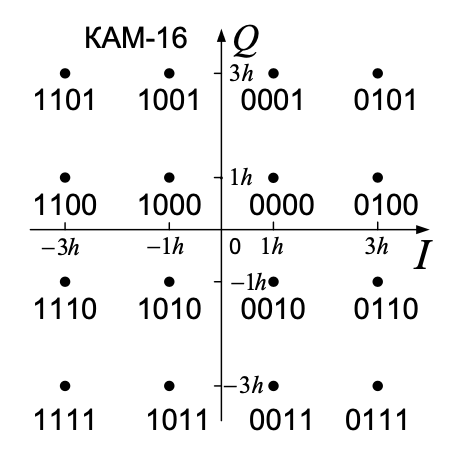
\includegraphics[scale=0.6]{cam_16}
    \caption{Сигнальное созвездие для КАМ-16} 
    \label{fig:cam_16}
  \end{figure}

  \item Изобразить график реализации $c(t)$ случайного процесса
  $C(t)$, формируемого с выхода блока сверточного кодера (К). 
  Реализация $с(t)$ поступает на вход блока ФМС на первых 
  16 бинарных интервалах длительностью $T_B$. 
  Написать аналитическое выражение для 
  случайного процесса $C(t)$.
  \begin{figure}[H]
    \centering
    \begin{tikzpicture}[x=0.8cm, y=-1cm]
      \draw[->, very thick] (0,1) -- (16.2,1);
      \draw[->, very thick] (0,2.2) -- (0,-0.2);

      \draw (0,0) -- (3,0) -- (3,2);
      \draw (3,2) -- (7,2) -- (7,0);
      \draw (7,0) -- (9,0) -- (9,2);
      \draw (9,2) -- (10,2) -- (10,0);
      \draw (10,0) -- (11,0) -- (11,2);
      \draw (11,2) -- (13,2) -- (13,0);
      \draw (13,0) -- (16,0);

      \node at (0.5,-0.5) {$1$};
      \node at (1.5,-0.5) {$1$};

      \node at (2.5,-0.5) {$1$};
      \node at (3.5,-0.5) {$0$};

      \node at (4.5,-0.5) {$0$};
      \node at (5.5,-0.5) {$0$};

      \node at (6.5,-0.5) {$0$};
      \node at (7.5,-0.5) {$1$};

      \node at (8.5,-0.5) {$1$};
      \node at (9.5,-0.5) {$0$};

      \node at (10.5,-0.5) {$1$};
      \node at (11.5,-0.5) {$0$};

      \node at (12.5,-0.5) {$0$};
      \node at (13.5,-0.5) {$1$};

      \node at (14.5,-0.5) {$1$};
      \node at (15.5,-0.5) {$1$};
    \end{tikzpicture}
    \caption{График реализации $c(t)$ с выхода сверточного кодера}
  \end{figure}

  \[ C(t)=\sum^\infty_{n=-\infty}C_n\cdot g_1(t-nT_B) \]
  где $g_1(t)$ -- прямоугольный импульс длительностью $T_B$.
  \[ g_1(t)=\begin{cases}
    1\,В, & 0\leq t \leq T_B;\\
    0\,В, & t<0,\,t>T_B,
  \end{cases} \]
  где $g_1(t-nT_B)$ -- прямоугольный импульс такой же формы, 
  как и $g_1(t)$, но сдвинутый вправо относительно импульса 
  $g_1(t)$ на величину $nT_B$, если $n>0$, или 
  влево, если $n<0$; 
  
  $C_n$ -- численный коэффициент, являющийся реализацией 
  случайной величины $C_n$ на $n$-интервале $T_B$.
  Величина $C_n$ принимает два дискретных значения $h(B)$ и 
  $-h(B)$ с вероятностью $0,5$ каждое, \mbox{т. е.} 
  \[ P(h)=P(-h)=0,5. \]

  Если в заданной реализации $c(t)$ на $n$-интервале передается 
  информационный символ «1», то $c_n=h(B)$, 
  если передается символ «0», то $c_n=-h(B)$.

  \item В соответствии с сигнальным созвездием модулятора КАМ-16 
  изобразить графики реализаций $i(t)$ и $q(t)$ на выходе 
  блока ФМС, соответствующие входной реализации $c(t)$. 
  Написать аналитические выражения для случайных процессов 
  $I(t)$ и $Q(t)$.
  \begin{equation} \label{eq:ItQt}
  I(t)=\sum^\infty_{n=-\infty}I_n\cdot g_2(t-nT_S);\,
  Q(t)=\sum^\infty_{n=-\infty}Q_n\cdot g_2(t-nT_S),
  \end{equation}
  где $g_(t)$ -- прямоугольный импульс длительностью 
  $T_S=4T_B$. $T_S$ -- символьный интервал; 
  $T_B$ -- бинарный интервал;
  \[ g_2(t)=\begin{cases}
    1\,В, & 0\leq t \leq T_B;\\
    0\,В, & t<0,\,t>T_B,
  \end{cases} \]
  где $g_2(t-nT_S)$ -- прямоугольный импульс такой же формы, 
  как и $g_2(t)$, но сдвинутый вправо относительно импульса 
  $g_2(t)$ на величину $nT_S$, если $n>0$, или 
  влево, если $n<0$;
  
  $I_n$ и $Q_n$ -- независимые случайные величины, заданные на 
  символьном интервале с номером $n$, 
  которые согласно сигнальному созвездию (рис. \ref{fig:cam_16})
  принимают четыре дискретных значения 
  $-3h,\, -h,\, h,\, 3h$ с вероятностью 0,25 каждое, т. е.
  \[ P(-3h)=P(-h)=P(h)=P(3h)=0,25. \]

  \begin{figure}[H]
    \centering
    \begin{tikzpicture}[x=0.8cm, y=-0.8cm]
      \draw[->, very thick] (0,2) -- (16.2,2);
      \draw[->, very thick] (0,4.2) -- (0,-0.2);

      \node at (-0.5,0) [left] {$3h$};
      \node at (-0.5,1) [left] {$h$};
      \node at (-0.5,2) [left] {$0$};
      \node at (-0.5,3) [left] {$-h$};
      \node at (-0.5,4) [left] {$-3h$};

      \draw (0,4) -- (4,4) -- (4,1);
      \draw (4,1) -- (8,1) -- (8,3);
      \draw (8,3) -- (12,3) -- (12,0);
      \draw (12,0) -- (16,0);
    \end{tikzpicture}
    \caption{График реализации $i(t)$}
  \end{figure}

  \begin{figure}[H]
    \centering
    \begin{tikzpicture}[x=0.8cm, y=-0.8cm]
      \draw[->, very thick] (0,2) -- (16.2,2);
      \draw[->, very thick] (0,4.2) -- (0,-0.2);

      \node at (-0.5,0) [left] {$3h$};
      \node at (-0.5,1) [left] {$h$};
      \node at (-0.5,2) [left] {$0$};
      \node at (-0.5,3) [left] {$-h$};
      \node at (-0.5,4) [left] {$-3h$};

      \draw (0,3) -- (4,3) -- (4,0);
      \draw (4,0) -- (8,0) -- (8,3);
      \draw (8,3) -- (12,3) -- (12,4);
      \draw (12,4) -- (16,4);
    \end{tikzpicture}
    \caption{График реализации $q(t)$}
  \end{figure}

  \item Написать аналитические выражения для корреляционной 
  функции $B_C(\tau)$ и спектральной плотности мощности 
  $G_C(\omega)$ входного случайного процесса $C(t)$ 
  и построить графики этих функций.

  Процесс $C(t)$ является случайным синхронным телеграфным сигналом. Его корреляционная функция имеет вид:
  \[ B_C(\tau)=\begin{cases}
    h^2(1-\frac{|\tau|}{T}),&|\tau|\leq T\\
    0, & |\tau| > T
  \end{cases}, \]
  а спектральная плотность мощности
  \[ G_C(\omega)
  =\int^\infty_{-\infty}B_C(\tau)e^{-i\omega\tau}d\tau
  =\int^\infty_{-\infty}B_C(\tau)\cos{\omega\tau}d\tau
  =T\cdot h^2\cdot\frac{\sin^2(\frac{\omega T}{2})}{(\frac{\omega T}{2})^2}, \]
  где $T=T_B$ -- длительность тактового интервала.
  \begin{figure}[H]
    \centering
    \begin{tikzpicture}
      \pgfmathsetmacro{\T}{1.8}
      \pgfmathsetmacro{\h}{1}
      \begin{axis}[
        width=10cm,height=6cm,
        axis lines = left,
        ylabel = {$B_C(\tau)$},
        xlabel = {$\tau$},
      ]
        \addplot [
          color=blue,
          samples=100,
        ]
        {\h^2*(1-abs(x)/\T)};
      \end{axis}
    \end{tikzpicture}
    \caption{График корреляционной функции $B_C(\tau)$}
  \end{figure}

  \begin{figure}[H]
    \centering
    \begin{tikzpicture}
      \pgfmathsetmacro{\T}{1.8}
      \pgfmathsetmacro{\h}{1}
      \begin{axis}[
        width=10cm,height=6cm,
        axis lines = left,
        ylabel = {$G_C(\omega)$},
        xlabel = {$\omega$},
      ]
        \addplot [
          color=blue,
          samples=100,
          domain=-400:400,
        ]
        {\h^2*\T*(sin(x*\T/2)^2)/(x*\T/2)^2};
      \end{axis}
    \end{tikzpicture}
    \caption{График спектральной плотности мощности 
    $G_C(\omega)$}
  \end{figure}

  \item Написать аналитические выражения для 
  корреляционных функций $B_I(\tau)$ и $B_Q(\tau)$, 
  спектральных плотностей мощности $G_I(\omega)$ 
  и $G_Q(\omega)$ случайных процессов $I(t)$ и $Q(t)$. 
  Построить графики этих функций.

  Процессы $I(t)$ и $Q(t)$ будут иметь идентичные друг другу корреляционные функции и спектральные плотности 
  мощности, поскольку они оба отличаются от процесса 
  $C(t)$ лишь длительностью сигнального интервала 
  $T_S=4T_B$.
  \[ B_I(0)=B_Q(0)=D\{I(t)\}=D\{Q(t)\} \]
  \[ G_I(0)=G_Q(0)=\frac{D\{I(t)\}}{T_S}=\frac{D\{Q(t)\}}{T_S} \]
  \begin{align*}\begin{split}
    D\{I(t)\}=D\{Q(t)\}&
    =\sum^4_{n=1}(i_n-\overline{I_n(t)})^2\cdot P(i_n)\\
    &=0,25(-3h)^2+0,25(-h)^2+0,25h^2+0,25(3h)^2=5h^2
  \end{split}\end{align*}
  Корреляционные функции:
  \[ B_I(\tau)=B_Q(\tau)=\begin{cases}
    5h^2(1-\frac{|\tau|}{T_B}), & |\tau|\leq T_B\\
    0, & |\tau| > T_B
  \end{cases} \]
  Энергетический спектр:
  \[ G_I(\omega)=G_Q(\omega)
  =\int^\infty_{-\infty}B_C(\tau)e^{-i\omega\tau}d\tau
  =T\cdot h^2\cdot\frac{\sin^2(\frac{\omega T}{2})}{(\frac{\omega T}{2})^2} \]
  \begin{figure}[H]
    \centering
    \begin{tikzpicture}
      \pgfmathsetmacro{\T}{1.8*4}
      \pgfmathsetmacro{\h}{1}
      \begin{axis}[
        width=10cm,height=6cm,
        axis lines = left,
        ylabel = {$B(\tau)$},
        xlabel = {$\tau$},
      ]
        \addplot [
          color=red,
          samples=100,
        ]
        {5*\h^2*(1-abs(x)/\T)};
      \end{axis}
    \end{tikzpicture}
    \caption{График корреляционной функции 
    $B_I(\tau)$, $B_Q(\tau)$}
  \end{figure}

  \begin{figure}[H]
    \centering
    \begin{tikzpicture}
      \pgfmathsetmacro{\T}{1.8*4}
      \pgfmathsetmacro{\h}{1}
      \begin{axis}[
        width=10cm,height=6cm,
        axis lines = left,
        ylabel = {$G(\omega)$},
        xlabel = {$\omega$},
      ]
        \addplot [
          color=red,
          samples=100,
          domain=-200:200,
        ]
        {\h^2*\T*(sin(x*\T/2)^2)/(x*\T/2)^2};
      \end{axis}
    \end{tikzpicture}
    \caption{График спектральной плотности мощности 
    $G_I(\omega)$, $G_Q(\omega)$}
  \end{figure}

  \item Сравнить графики корреляционных функций и спектральных 
  плотностей мощности сигналов на входе и выходе блока ФМС. 
  Привести краткое описание результатов сравнения и, 
  используя общие положения теории преобразования Фурье, 
  пояснить, почему спектр выходных сигналов уже спектра входного 
  сигнала.

  \begin{figure}[H]
    \centering
    \begin{tikzpicture}
      \pgfmathsetmacro{\T}{1.8}
      \pgfmathsetmacro{\TB}{1.8*4}
      \pgfmathsetmacro{\h}{1}
      \begin{axis}[
        width=10cm,height=6cm,
        axis lines = left,
        ylabel = {$B(\tau)$},
        xlabel = {$\tau$},
      ]
        \addplot [
          color=blue,
          samples=100,
          domain=-\T:\T,
        ]
        {\h^2*(1-abs(x)/\T)};
        \addlegendentry{$B_C(\tau)$};
        \addplot [
          color=red,
          samples=100,
          domain=-\TB:\TB,
        ]
        {5*\h^2*(1-abs(x)/\TB)};
        \addlegendentry{$B_I(\tau)$, $B_Q(\tau)$};
      \end{axis}
    \end{tikzpicture}
    \caption{Графики корреляционной функции $B_C(\tau)$ и $B_I(\tau)$}
  \end{figure}

  \begin{figure}[H]
    \centering
    \begin{tikzpicture}
      \pgfmathsetmacro{\T}{1.8}
      \pgfmathsetmacro{\TB}{1.8*4}
      \pgfmathsetmacro{\h}{1}
      \begin{axis}[
        width=10cm,height=6cm,
        axis lines = left,
        ylabel = {$G(\omega)$},
        xlabel = {$\omega$},
      ]
        \addplot [
          color=blue,
          samples=100,
          domain=-300:300,
        ]
        {\h^2*\T*(sin(x*\T/2)^2)/(x*\T/2)^2};
        \addlegendentry{$G_C(\omega)$};
        \addplot [
          color=red,
          samples=100,
          domain=-300:300,
        ]
        {\h^2*\TB*(sin(x*\TB/2)^2)/(x*\TB/2)^2};
        \addlegendentry{$G_I(\omega)$, $G_Q(\omega)$};
      \end{axis}
    \end{tikzpicture}
    \caption{График спектральной плотности мощности 
    $G_C(\omega)$ и $G_I(\omega)$}
  \end{figure}

  Выходной спектр уже, поскольку функция $G(\omega)$ равна
  0 при значениях $\omega = n/T$, а $T_S=4T_B$, поэтому
  изгибы встречаются в 4 раза чаще.
\end{enumerate}

\subsection{Модулятор}
В состав модулятора структурной схемы цифровой системы связи (ЦСС), 
рис. \ref{fig:struct_scheme}, между блоками ФМС и перемножителями 
входят сглаживающие формирующие фильтры СФФ, необходимые для 
оптимизации ЦСС в отношении межсимвольной помехи, а также инвертор и 
сумматор, на выходе которого получаем сигнал заданного вида модуляции.

\subsubsection{Сглаживающий формирующий фильтр}
\begin{figure}
  \centering
  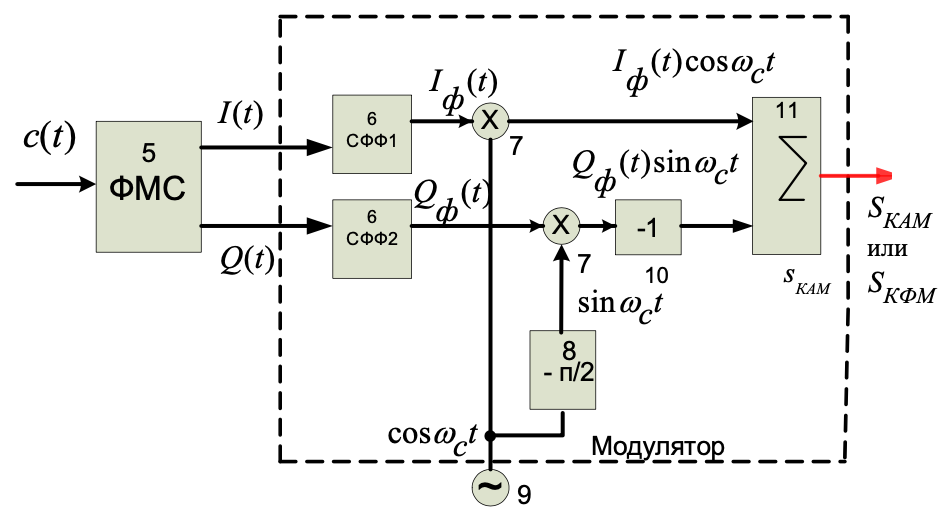
\includegraphics[scale=0.6]{modulator}
  \caption{Структурная схема модулятора}
  \label{fig:modulator}
\end{figure}
Требуется:
\begin{enumerate}
  \item Изобразить структурную схему модулятора в составе ЦСС 
  (рис. \ref{fig:modulator}).

  \item Написать аналитические выражения для сигнала $x(t)$ 
  со <<спектром приподнятого косинуса>> (импульса Найквиста) 
  и его спектральной плотности $S_x(f)$ для значений коэффициента 
  сглаживания $0\leq \beta \leq 1$. Изобразить графики сигналов 
  $x(t)$ и соответствующие спектральные плотности 
  при $0\leq \beta \leq 1$.

  Импульсы Найквиста $x(t)$ и их спектральные плотности $S_x(f)$
  характеризуются следующими аналитическими выражениями:
  \begin{equation} \label{eq:imp_niq}
    x(t)=\frac{\sin(\frac{\pi\cdot t}{T})}{\frac{\pi\cdot t}{T}}
    \cdot\frac{\cos(\frac{\pi\beta t}{T})}{1-\frac{4\beta^2 t^2}{T^2}}; 
  \end{equation}

  \begin{equation}  
    S_x(f)=\begin{cases}
      T, & 0\leq |f|\leq\dfrac{1-f}{2T};\\[10pt]
      \dfrac{T}{2}\cdot\biggr\{1+\cos\biggr[\dfrac{\pi T}{\beta}
      \cdot\biggr(|f|-\dfrac{1-\beta}{2T}\biggr)\biggr]\biggr\}, &
      \biggr(\dfrac{1-f}{2T}\biggr)\leq|f|\leq 
      \biggr(\dfrac{1+f}{2T}\biggr);\\[10pt]
      0, & |f|>\dfrac{1+f}{2T},
    \end{cases}
  \end{equation}
  где $\beta$ -- коэффициент сглаживания (или ската), который 
  может принимать значения в интервале $0\leq \beta \leq 1$.

  \begin{figure}[H]
    \centering
    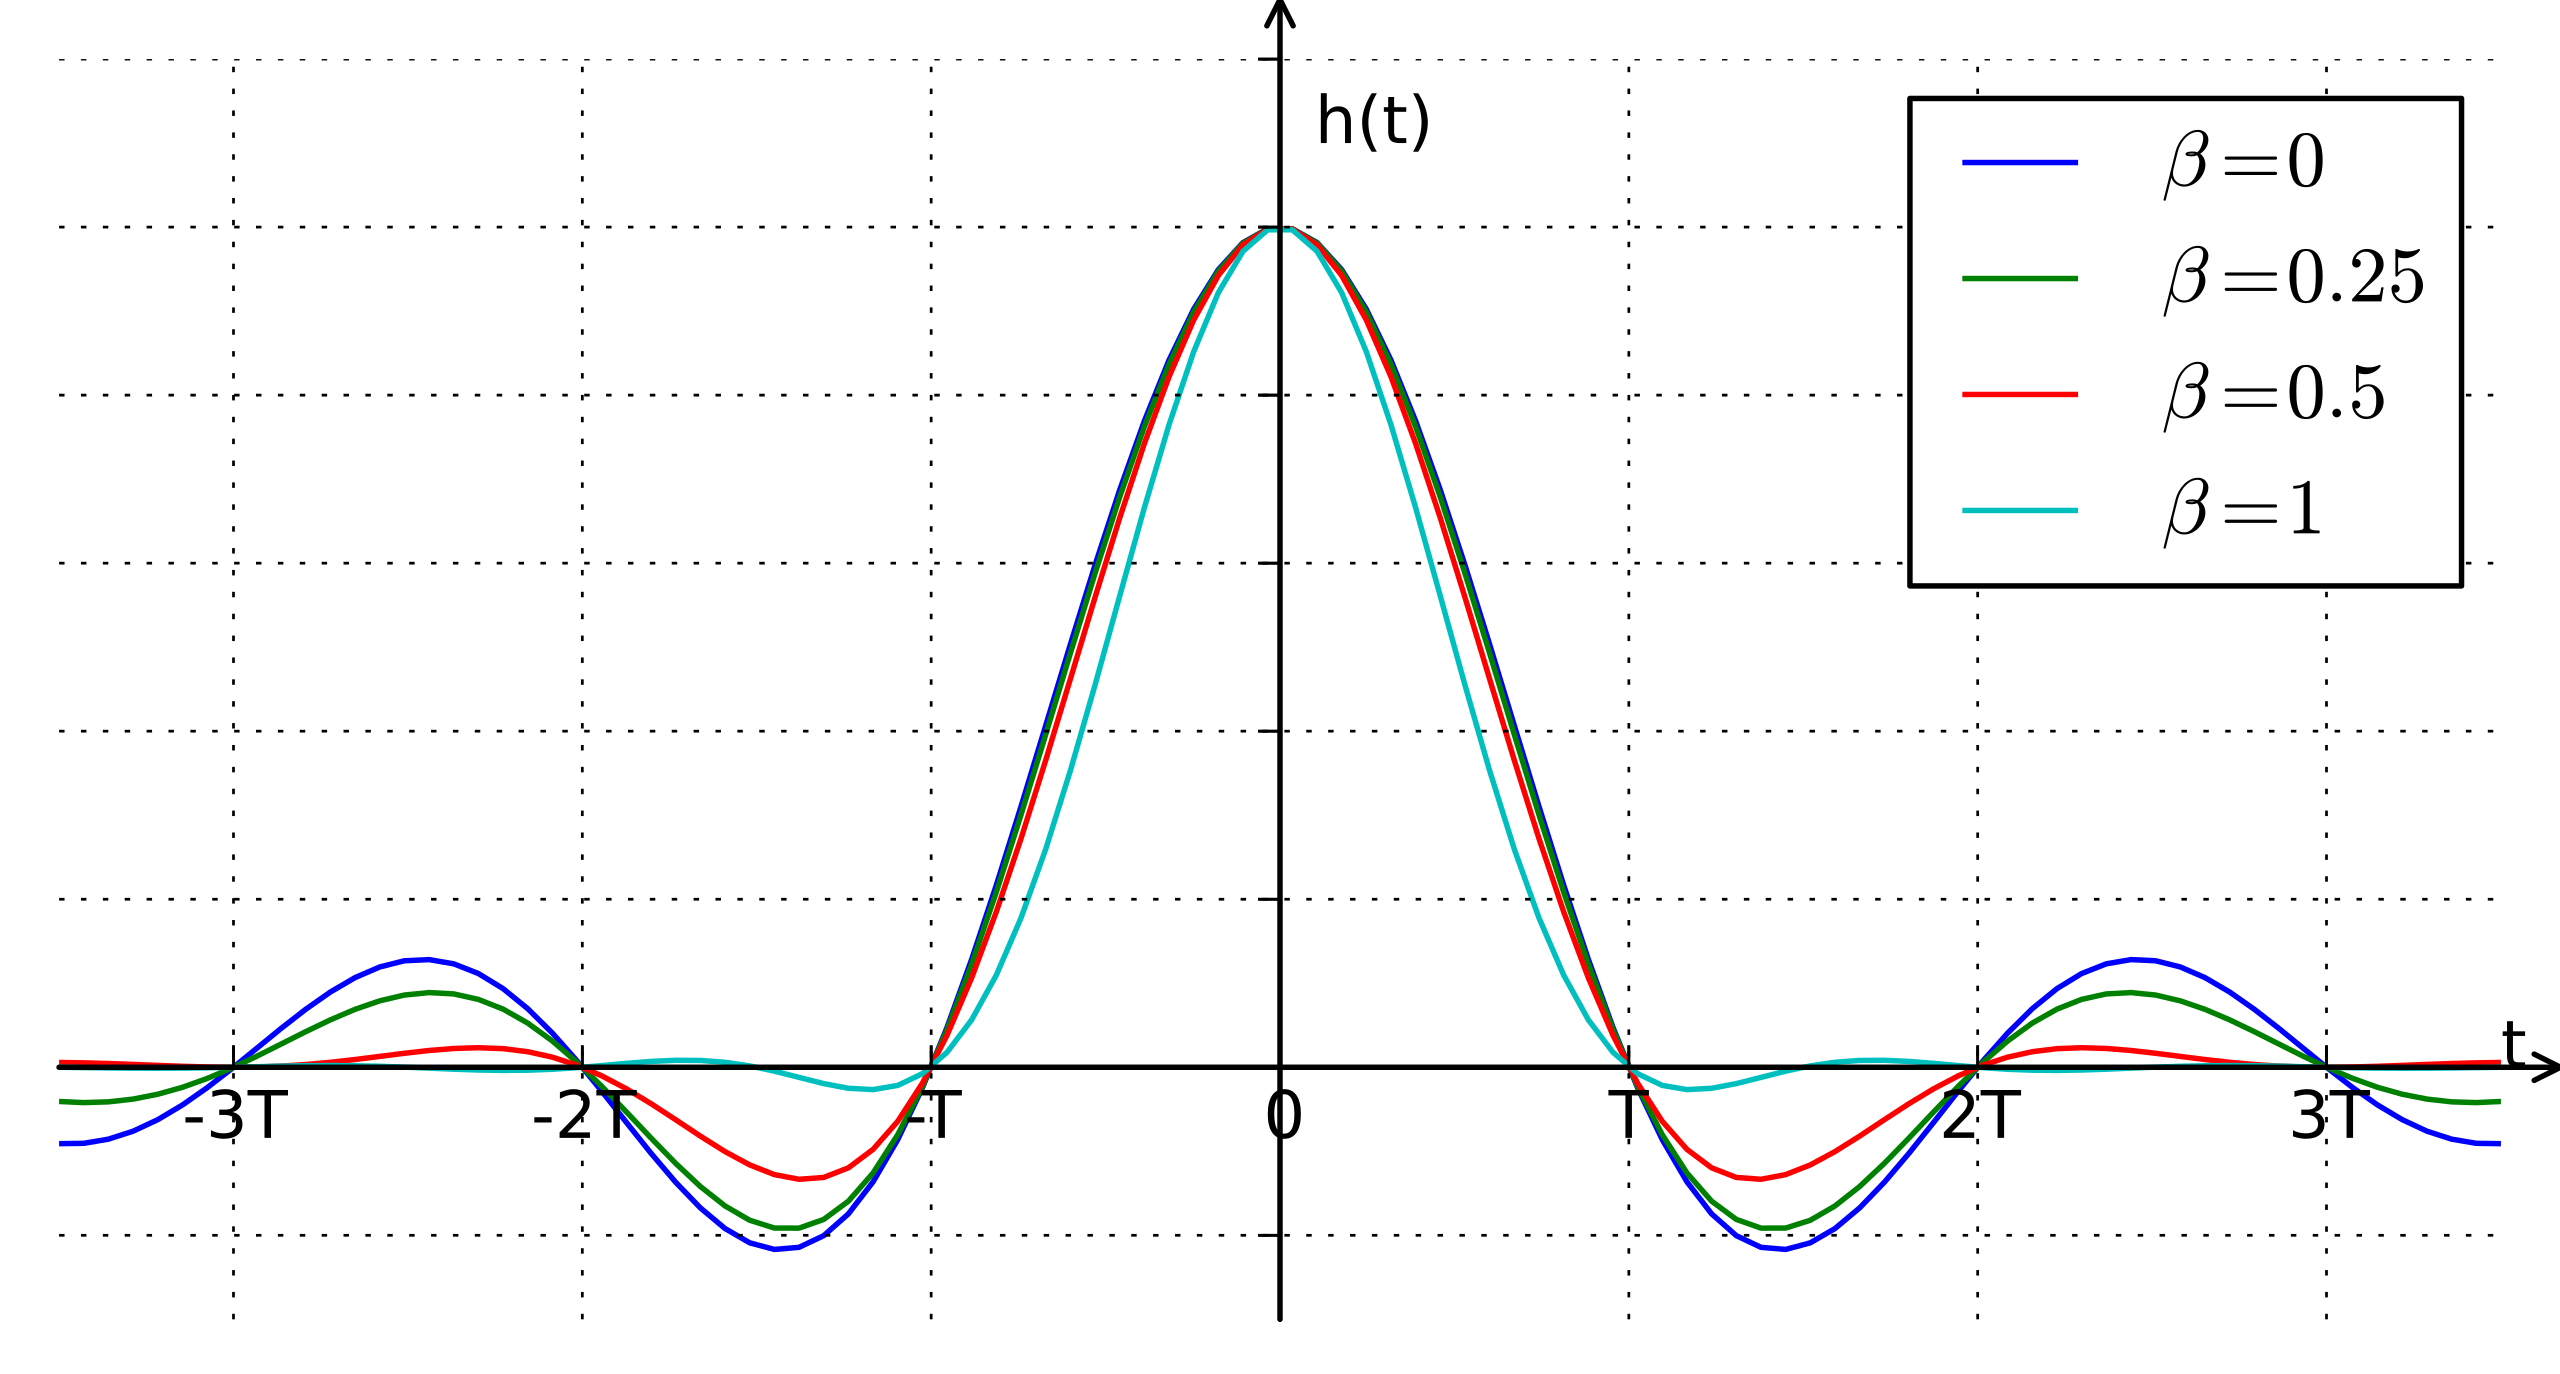
\includegraphics[scale=0.13]{Raised-cosine-impulse}
    \caption{График импульсов Найквиста $x(t)$} 
    \label{fig:imp_niq}
  \end{figure}

  \begin{figure}[H]
    \centering
    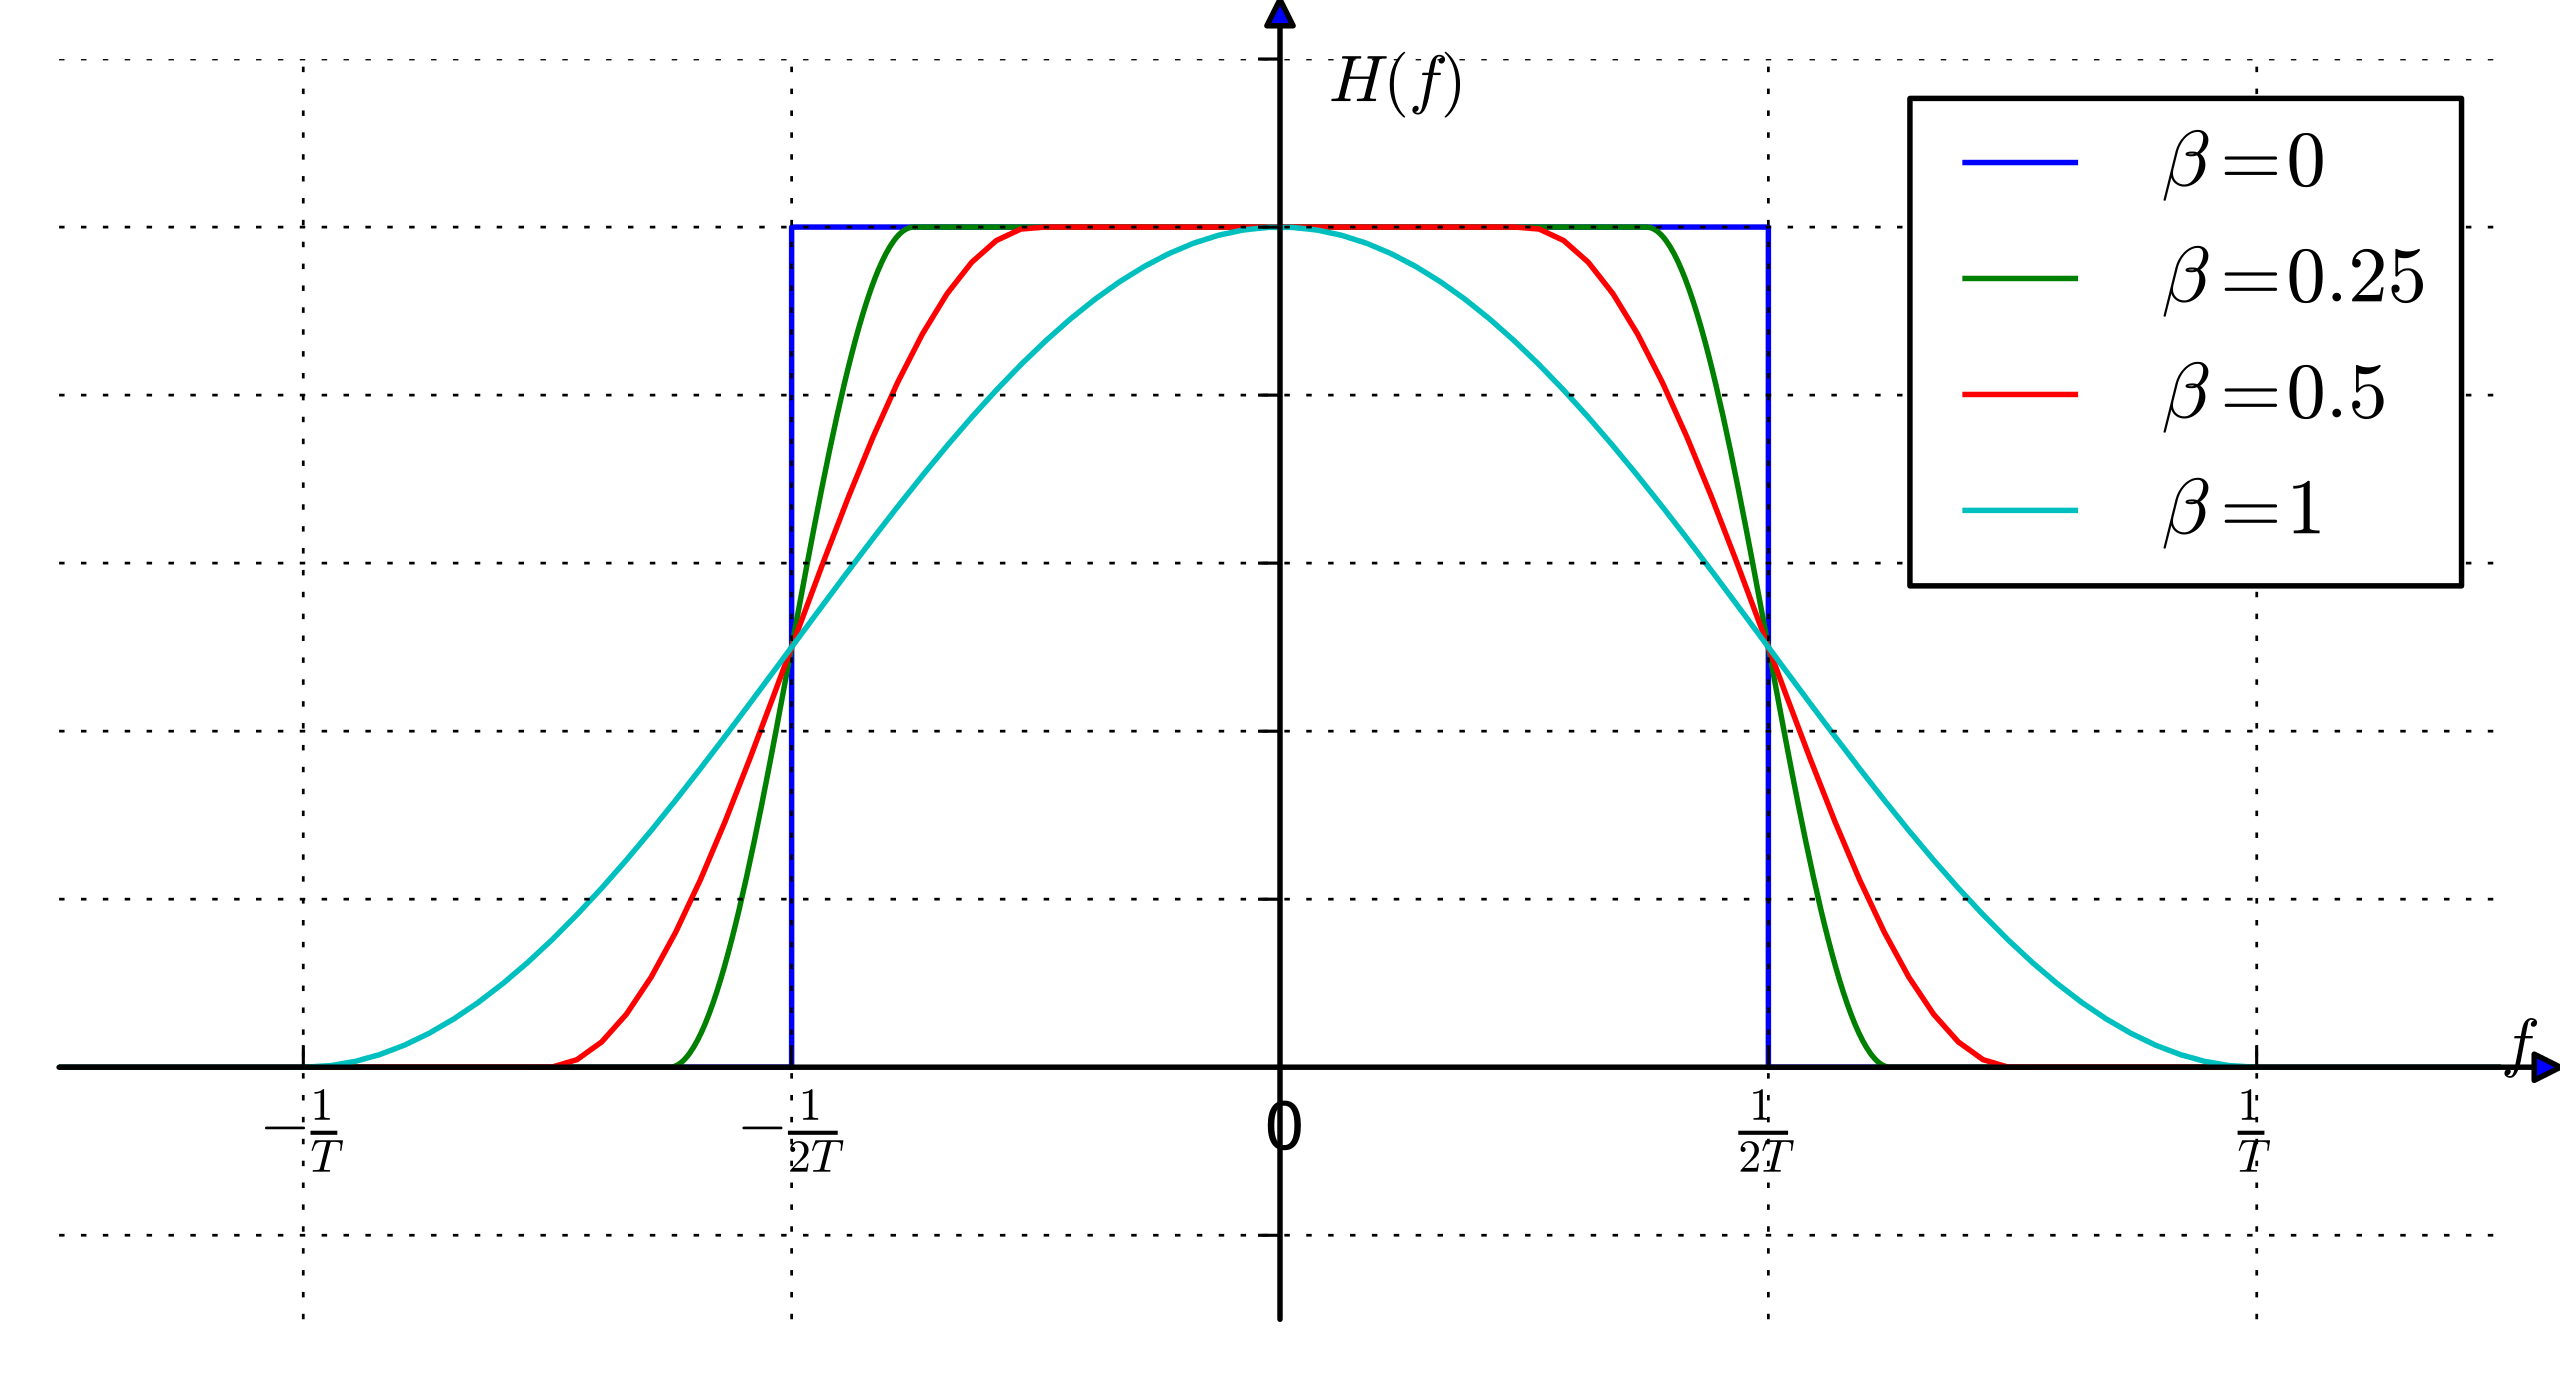
\includegraphics[scale=0.13]{Raised_cosine_filter}
    \caption{График спектральных плотностей $S_x(f)$}
  \end{figure}

  \item На одном рисунке изобразить графики спектральных плотностей 
  $S_x(\omega)$ и $S_{x1}(\omega)$ сигналов $x(t)$ и $x_1(t)$, 
  где $x(t)$ -- импульс Найквиста при коэффициенте сглаживания 
  $\beta=1$; $x_1(t)$ – импульс со спектральной плотностью 
  $S_{x1}(\omega)=\sqrt{S_x(\omega)}$.

  \begin{figure}[H]
    \centering
    \begin{tikzpicture}
      \pgfmathsetmacro{\PI}{3.14}
      \pgfmathsetmacro{\T}{1.8}
      \begin{axis}[
        width=10cm,height=6cm,
        axis lines = left,
        ylabel = {$S(\omega)$},
        xlabel = {$\omega$},
        domain=-32:32,
      ]
        \addplot [
          color=blue,
          samples=100,
        ]
        {\T/2*(1+cos(\PI*\T*abs(x)))};
        \addlegendentry{$S_x(\omega)$};
        \addplot [
          color=red,
          samples=100,
        ]
        {sqrt(\T/2*(1+cos(\PI*\T*abs(x))))};
        \addlegendentry{$S_{x1}(\omega)$};
      \end{axis}
    \end{tikzpicture}
    \caption{Графики спектральных плотностей 
    $S_x(\omega)$ и $S_{x1}(\omega)$ сигналов $x(t)$ и $x_1(t)$}
  \end{figure}

  \item На одном рисунке изобразить графики импульсов 
  $x(t)$ и $x_1(t)$.

  \begin{figure}[H]
    \centering
    \begin{tikzpicture}
      \pgfmathsetmacro{\PI}{3.14}
      \pgfmathsetmacro{\T}{1}

      \begin{axis}[
        width=10cm,height=6cm,
        axis lines = left,
        ylabel = {$x(t)$},
        xlabel = {$t$},
        domain = -2:2,
      ]
        \addplot [no markers] gnuplot [
          color=blue,
          samples=100,
        ]
        {sin(\PI*x/\T)/\PI/x*\T*cos(\PI*x/\T)/(1-4*x^2/\T^2)};
        \addlegendentry{$x(t)$};
        \addplot [no markers] gnuplot [
          color=red,
          samples=100,
        ]
        {sin(\PI*x*1.27/\T)/\PI/x*1.27*\T*cos(\PI*x*1.27/\T)/(1-4*(x*1.27)^2/\T^2)};
        \addlegendentry{$x_1(t)$};
      \end{axis}
    \end{tikzpicture}
    \caption{Импульс Найквиста $x(t)$ и искомый импульс $x_1(t)$}
  \end{figure}
  \item Написать аналитические выражения для случайных процессов 
  $I_ф(t)$ и $Q_ф(t)$.
  \[ I_ф(t)=\sum^\infty_{n=-\infty}I_ng_3(t-nT), \]
  где $i_n$ -- детерминированная величина, которая является 
  реализацией случайной величины $I_n$. 
  Величины $i_n$ в выражениях для $i(t)$ и $i_ф(t)$ 
  принимают одинаковые значения на соответствующих символьных 
  интервалах $T$.

  \[ Q_ф(t)=\sum^\infty_{n=-\infty}Q_ng_3(t-nT), \]
  где $I_n(t)$ и $Q_n(t)$ -- независимые случайные величины, 
  принимающие известные дискретные значения с заданными 
  вероятностями, какие они имеют в формулах (\ref{eq:ItQt});

  $g_3(t)=x_{1н}(t-3T)$ -- детерминированный импульс,
  спектральная плотность которого выражается через спектральную 
  плотность импульса Найквиста.

  \item Написать аналитические выражения для корреляционных функций
  и спектральных плотностей мощности случайных процессов 
  $I_ф(t)$ и $Q_ф(t)$ и построить графики этих функций.

  \begin{equation}
    B_{I_ф}(\tau)=\frac{\overline{I_n^2}}{1,27^2}\cdot x(\tau),
  \end{equation}
  где $\overline{I^2_n}=5h^2$ для КАМ-16;

  $x(\tau)$ -- импульс Найквиста при значении $\beta=1$.

  Так как случайный процесс $Q_ф(t)$ на выходе нижнего сглаживающего 
  формирующего фильтра (СФФ) имеет такие же вероятностные 
  характеристики, как и процесс $I_ф(t)$, то можно написать 
  следующие равенства:
  \begin{equation}
      B_{Q_ф}(\tau)=B_{I_ф}(\tau);\,
      G_{Q_ф}(\omega)=G_{I_ф}(\omega).
  \end{equation}
  \begin{figure}[H]
    \centering
    \begin{tikzpicture}
      \pgfmathsetmacro{\PI}{3.14}
      \pgfmathsetmacro{\T}{1}

      \begin{axis}[
        width=10cm,height=6cm,
        axis lines = left,
        ylabel = {$B(\tau)$},
        xlabel = {$\tau$},
        domain = -2:2,
      ]
        \addplot [no markers] gnuplot [
          color=blue,
          samples=100,
        ]
        {sin(\PI*x/\T)/\PI/x*\T*cos(\PI*x/\T)/(1-4*x^2/\T^2)};
      \end{axis}
    \end{tikzpicture}
    \caption{График корреляционных функций 
    $B_{I_ф}(\tau)$ и $B_{Q_ф}(\tau)$
    случайных процессов $I_ф(t)$ и $Q_ф(t)$}
  \end{figure}
  \begin{equation}
    G_{I_ф}(\omega)=\begin{cases}
      \dfrac{\overline{I^2_n}}{1,27^2}\cdot\dfrac T2
      \biggr[1+\cos\biggr(\omega\dfrac T2\biggr)\biggr],
      &|\omega|\leq \dfrac{2\pi}{T};\\[14pt]
      0, & |\omega|>\dfrac{2\pi}{T}.
    \end{cases}
  \end{equation}
  \begin{figure}[H]
    \centering
    \begin{tikzpicture}
      \pgfmathsetmacro{\PI}{3.14}
      \pgfmathsetmacro{\T}{1.8}
      \begin{axis}[
        width=10cm,height=6cm,
        axis lines = left,
        ylabel = {$S(\omega)$},
        xlabel = {$\omega$},
        domain=-32:32,
      ]
        \addplot [
          color=blue,
          samples=100,
        ]
        {\T/2*(1+cos(\PI*\T*abs(x)))};
      \end{axis}
    \end{tikzpicture}
    \caption{График спектральных плотностей мощности
    $G_{I_ф}(\omega)$ и $G_{Q_ф}(\omega)$}
  \end{figure}
\end{enumerate}

\subsubsection{Блоки перемножителей, инвертор, сумматор}
Требуется:
\begin{enumerate}
  \item Написать аналитические выражения для корреляционных функций
  $B_{I_ф\cos}(\tau)$ и $B_{Q_ф\sin}(\tau)$ случайных сигналов
  $I_ф(t)\cdot\cos(\omega_Ct+\varphi_C)$ и 
  $Q_ф(t)\cdot\sin(\omega_Ct+\varphi_C)$ на выходах перемножителей,
  где $\varphi_C$ -- случайная фаза с равномерной плотностью 
  вероятности на интервале $0...2\pi$. 
  Случайная фаза $\varphi_C$ не зависит от случайных процессов 
  $I_ф(t)$ и $Q_ф(t)$.

  \begin{equation}
    B_{I_ф\cos}(\tau)=B_{Q_ф\sin}(\tau)=\frac 12B_{I_ф}(\tau)\cdot\cos\omega_c\tau,
  \end{equation}
  где $\tau=(t_2-t_1)$.

  \item Написать аналитические выражения для корреляционных 
  функций $B_S(\tau)=B_{I_ф}(\tau)\cdot\cos\omega_C\tau
  =B_{Q_ф}(\tau)\cdot\cos\omega_C\tau$ и для спектральной
  плотности мощности $G_S(\omega)$ сигнала $S(t)$ на
  выходе сумматора. Построить графики этих функций.
  \begin{equation} \label{eq:BSTau}
    B_S(\tau)=\overline{I^2_n}\cdot\frac{1}{1,27^2}\cdot x(\tau)
    \cdot\cos\omega_C\tau,
  \end{equation}
  где $x(\tau)$ -- импульс Найквиста, определяемый 
  (\ref{eq:imp_niq}) при $\beta=1$ (рис. \ref{fig:imp_niq});

  $\overline{I^2_n}=5h^2$ для КАМ-16.
  
  Спектральная плотность мощности $G_S(\omega)$ случайного сигнала 
  $S(t)$ в соответствии с теоремой Винера -- Хинчина определяется 
  через преобразование Фурье корреляционной функции $B_S(\tau)$.
  Используя (\ref{eq:BSTau}), получим:
  \begin{equation}
    \begin{split}
      G_S(\omega)&=\int^\infty_{-\infty}B_{I_ф\cos}(\tau)
      \cdot e^{-i\omega\tau}d\tau
      =\overline{I^2_n}\cdot\frac{1}{1,27^2}
      \int^\infty_{-\infty}x(\tau)\cdot\cos\omega_C\tau
      \cdot e^{-i\omega\tau}d\tau\\
      &=\frac 12 \cdot \frac{\overline{I^2_n}}{1,27^2}
      [S_x(\omega-\omega_C)+S_x(\omega+\omega_C)],
    \end{split}
  \end{equation}
  Учитывая, что функция $S_x(\omega)$ импульса Найквиста $x(t)$
  при значении $\beta=1$ и $f=\frac{\omega}{2\pi}$ равна
  \begin{equation}
    S_x(\omega)=\begin{cases}
      \dfrac T2\biggr(1+\cos\dfrac T2\omega\biggr), 
      & |\omega|\leq\dfrac{2\pi}{T};\\[10pt]
      0, & |\omega|>\dfrac{2\pi}{T}.
    \end{cases}
  \end{equation}
  Спектральная плотность $G_S(\omega)$ на выходе сумматора будет 
  равна удвоенной спектральной плотности $G_{I_ф\cos}(\omega)$.

  \begin{figure}[H]
    \centering
    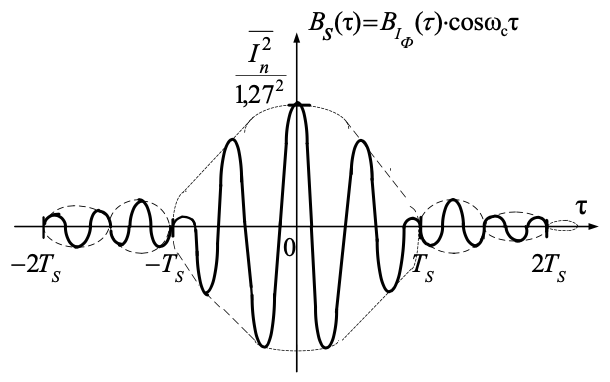
\includegraphics{BSTau}
    \caption{График корреляционной функции $B_S(\tau)$}
  \end{figure}

  \begin{figure}[H]
    \centering
    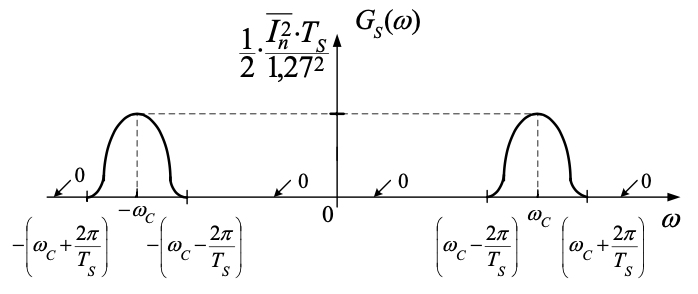
\includegraphics{GSOmega}
    \caption{Спектральные плотности мощности $G_S(\omega)$}
  \end{figure}
\end{enumerate}

\subsection{Непрерывный канал}
Передача сигнала $S(t)$ происходит по непрерывному неискажающему 
каналу с постоянными параметрами в присутствии аддитивной помехи
$n(t)$ типа гауссовского белого шума. Сигнал $Z(t)$ на выходе такого 
канала имеет вид
\begin{equation}
  Z(t)=\mu\cdot S(t)+n(t),
\end{equation}
где $\mu=1$ -- коэффициент передачи канала. 

Односторонняя спектральная плотность мощности помехи $n(t)$ 
равна $N_0=2,3\cdot 10^{-7}\,В^2/Гц$.

Требуется:
\begin{enumerate}
  
\end{enumerate}

\subsection{Декодер}
По каналу передавался код 
\(\overline{u}=11 10 00 01 10 10 01 11 11...\).
Ошибка произошла на тактовом интервале \(q=3\).
Таким образом, на вход декодера поступает последовательность 
\(\overline{Z}=11 \overset{\times}{0} 0 00 01 10 10 01 11 11...\). Крестиком обозначен ошибочно принятый символ.

\subsubsection{Диаграмма декодера}
\begin{figure}
  \begin{tikzpicture}[x=1.2cm, y=-1cm]

    \node at (-0.5,0) [left] {$s_1=00$};
    \node at (-0.5,1) [left] {$s_2=10$};
    \node at (-0.5,2) [left] {$s_3=01$};
    \node at (-0.5,3) [left] {$s_4=11$};

    % Nodes
    \foreach \x in {0,...,9} {
      \node at (\x,-.7) {$\x$};
      \foreach \y in {0,...,3} {
        \node (s\x\y) at (\x,\y) [circle,fill=black,scale=0.7] {};
      }
    }

    \node at (0,0) [highlight] {};
    \node at (1,0) [highlight,label=left:{$2$}] {};
    \node at (1,1) [highlight,label=left:{$0$}] {};

    \node at (2,0) [highlight,label=left:{$0$}] {};
    \node at (2,1) [highlight,label=left:{$2$}] {};
    \node at (2,2) [highlight,label=left:{$1$}] {};
    \node at (2,3) [highlight,label=left:{$1$}] {};

    \node at (3,0) [highlight,label=left:{$\frac{0}{2}$}] {};
    \node at (3,1) [highlight,label=left:{$\frac{2}{0}$}] {};
    \node at (3,2) [highlight,label=left:{$\frac{1}{1}$}] {};
    \node at (3,3) [highlight,label=left:{$\frac{1}{1}$}] {};

    \node at (4,0) [highlight,label=left:{$\frac{1}{1}$}] {};
    \node at (4,1) [highlight,label=left:{$\frac{1}{1}$}] {};
    \node at (4,2) [highlight,label=left:{$\frac{2}{0}$}] {};
    \node at (4,3) [highlight,label=left:{$\frac{0}{2}$}] {};

    \node at (5,0) [highlight,label=left:{$\frac{1}{1}$}] {};
    \node at (5,1) [highlight,label=left:{$\frac{1}{1}$}] {};
    \node at (5,2) [highlight,label=left:{$\frac{0}{2}$}] {};
    \node at (5,3) [highlight,label=left:{$\frac{2}{0}$}] {};

    \node at (6,0) [highlight,label=left:{$\frac{1}{1}$}] {};
    \node at (6,1) [highlight,label=left:{$\frac{1}{1}$}] {};
    \node at (6,2) [highlight,label=left:{$\frac{0}{2}$}] {};
    \node at (6,3) [highlight,label=left:{$\frac{2}{0}$}] {};

    \node at (7,0) [highlight,label=left:{$\frac{1}{1}$}] {};
    \node at (7,1) [highlight,label=left:{$\frac{1}{1}$}] {};
    \node at (7,2) [highlight,label=left:{$\frac{2}{0}$}] {};
    \node at (7,3) [highlight,label=left:{$\frac{0}{2}$}] {};

    \node at (8,0) [highlight,label=left:{$\frac{2}{0}$}] {};
    \node at (8,1) [highlight,label=left:{$\frac{0}{2}$}] {};
    \node at (8,2) [highlight,label=left:{$\frac{1}{1}$}] {};
    \node at (8,3) [highlight,label=left:{$\frac{1}{1}$}] {};

    \node at (9,0) [highlight,label=left:{$\frac{2}{0}$}] {};
    \node at (9,1) [highlight,label=left:{$\frac{0}{2}$}] {};
    \node at (9,2) [highlight,label=left:{$\frac{1}{1}$}] {};
    \node at (9,3) [highlight,label=left:{$\frac{1}{1}$}] {};

    % Edges
    \trellisEdges{0}{0}
    \trellisEdges{1}{0}
    \trellisEdges{1}{1}
    \foreach \x in {2,...,8} {
      \foreach \y in {0,...,3} {
        \trellisEdges{\x}{\y}
      }
    }

    % Inputs
    \node at (-0.5,4) [left, align=right] {Входная\\пара};

    \trellisIn{0}{11}
    \trellisIn{1}{00}
    \trellisIn{2}{00}
    \trellisIn{3}{01}
    \trellisIn{4}{10}
    \trellisIn{5}{10}
    \trellisIn{6}{01}
    \trellisIn{7}{11}
    \trellisIn{8}{11}
  \end{tikzpicture}

  \caption{Решетка декодера} \label{fig:decoder}
\end{figure}

\begin{figure}
  \begin{tikzpicture}[x=2cm, y=-1cm]

    \node at (-0.5,0) [left] {$s_1=00$};
    \node at (-0.5,1) [left] {$s_2=10$};
    \node at (-0.5,2) [left] {$s_3=01$};
    \node at (-0.5,3) [left] {$s_4=11$};

    % Nodes
    \foreach \x in {0,...,3} {
      \node at (\x,-.7) {$\x$};
      \foreach \y in {0,...,3} {
        \node (s\x\y) at (\x,\y) [circle,fill=black,scale=0.7] {};
      }
    }

    % Edges
    \trellisEdges{0}{0}
    \trellisEdges{1}{0}
    \trellisEdges{1}{1}
    \foreach \x in {2,...,2} {
      \foreach \y in {0,...,3} {
        \trellisEdges{\x}{\y}
      }
    }

    \draw[activeedge] (s00) -- (s10);
    \draw[activeedge] (s00) -- (s11);
    \draw[activeedge] (s10) -- (s20);
    \draw[activeedge] (s11) -- (s22);
    \draw[activeedge] (s20) -- (s30);
    \draw[activeedge] (s22) -- (s31);
    \draw[activeedge] (s11) -- (s23);
    \draw[activeedge] (s23) -- (s32);
    \draw[activeedge] (s23) -- (s33);

    \node at (0,0) [highlight] {};
    \node at (1,0) [highlight,label=left:{$2$}] {};
    \node at (1,1) [highlight,label=left:{$0$}] {};

    \node at (2,0) [highlight,label=left:{$0$}] {};
    \node at (2,1) [highlight,label=left:{$2$}] {};
    \node at (2,2) [highlight,label=left:{$1$}] {};
    \node at (2,3) [highlight,label=left:{$1$}] {};

    \node at (3,0) [highlight,label=left:{$\frac{0}{2}$}] {$\frac23$};
    \node at (3,1) [highlight,label=left:{$\frac{2}{0}$}] {$\frac41$};
    \node at (3,2) [highlight,label=left:{$\frac{1}{1}$}] {$\frac52$};
    \node at (3,3) [highlight,label=left:{$\frac{1}{1}$}] {$\frac52$};

    \node at (2.5,1) [text=red] {$\times$};
    \node at (2.5,0.5) [text=red] {$\times$};
    \node at (2.5,1.5) [text=red] {$\times$};
    \node at (2.5,2) [text=red] {$\times$};
    \node at (1.5,0.5) [text=red] {$\times$};

    % Inputs and Outputs
    \node at (-0.5,4) [left, align=right] {Входная\\пара};

    \trellisIn{0}{11}
    \trellisIn{1}{00}
    \trellisIn{2}{00}
  \end{tikzpicture}

  \caption{Сегмент решетки декодера от $t=0$, до $t=3$}
\end{figure}

\begin{figure}
  \begin{tikzpicture}[x=2cm, y=-1cm]

    \node at (-0.5,0) [left] {$s_1=00$};
    \node at (-0.5,1) [left] {$s_2=10$};
    \node at (-0.5,2) [left] {$s_3=01$};
    \node at (-0.5,3) [left] {$s_4=11$};

    % Nodes
    \foreach \x in {0,...,4} {
      \node at (\x,-.7) {$\x$};
      \foreach \y in {0,...,3} {
        \node (s\x\y) at (\x,\y) [circle,fill=black,scale=0.7] {};
      }
    }

    % Edges
    \trellisEdges{0}{0}
    \trellisEdges{1}{0}
    \trellisEdges{1}{1}
    \foreach \x in {2,...,3} {
      \foreach \y in {0,...,3} {
        \trellisEdges{\x}{\y}
      }
    }


    \draw[activeedge] (s00) -- (s11);
    \draw[activeedge] (s11) -- (s22);
    \draw[activeedge] (s22) -- (s31);
    \draw[activeedge] (s11) -- (s23);
    \draw[activeedge] (s23) -- (s32);
    \draw[activeedge] (s23) -- (s33);

    \draw[activeedge] (s31) -- (s43);
    \draw[activeedge] (s32) -- (s41);
    \draw[activeedge] (s32) -- (s40);
    \draw[activeedge] (s33) -- (s42);

    \node at (0,0) [highlight] {};
    \node at (1,0) [highlight,label=left:{$2$}] {};
    \node at (1,1) [highlight,label=left:{$0$}] {};

    \node at (2,0) [highlight,label=left:{$0$}] {};
    \node at (2,1) [highlight,label=left:{$2$}] {};
    \node at (2,2) [highlight,label=left:{$1$}] {};
    \node at (2,3) [highlight,label=left:{$1$}] {};

    \node at (3,0) [highlight,label=left:{$\frac{0}{2}$}] {};
    \node at (3,1) [highlight,label=left:{$\frac{2}{0}$}] {};
    \node at (3,2) [highlight,label=left:{$\frac{1}{1}$}] {};
    \node at (3,3) [highlight,label=left:{$\frac{1}{1}$}] {};

    \node at (2.5,1) [text=red] {$\times$};
    \node at (2.5,0.5) [text=red] {$\times$};
    \node at (2.5,1.5) [text=red] {$\times$};
    \node at (2.5,2) [text=red] {$\times$};
    \node at (1.5,0.5) [text=red] {$\times$};
    \node at (1.5,0) [text=red] {$\times$};
    \node at (0.5,0) [text=red] {$\times$};

    \node at (4,0) [highlight,label=left:{$\frac{1}{1}$}] {$\frac33$};
    \node at (4,1) [highlight,label=left:{$\frac{1}{1}$}] {$\frac33$};
    \node at (4,2) [highlight,label=left:{$\frac{2}{0}$}] {$\frac32$};
    \node at (4,3) [highlight,label=left:{$\frac{0}{2}$}] {$\frac14$};

    \node at (3.5,0) [text=red] {$\times$};
    \node at (3.5,0.5) [text=red] {$\times$};
    \node at (3.5,1.5) [text=red] {$\times$};
    \node at (3.5,3) [text=red] {$\times$};
    \node at (2.5,0) [text=red] {$\times$};

    % Inputs and Outputs
    \node at (-0.5,4) [left, align=right] {Входная\\пара};

    \trellisIn{0}{11}
    \trellisIn{1}{00}
    \trellisIn{2}{00}
    \trellisIn{3}{01}
  \end{tikzpicture}

  \caption{Сегмент решетки декодера от $t=0$, до $t=4$}
\end{figure}

\begin{figure}
  \begin{tikzpicture}[x=2cm, y=-1cm]

    \node at (-0.5,0) [left] {$s_1=00$};
    \node at (-0.5,1) [left] {$s_2=10$};
    \node at (-0.5,2) [left] {$s_3=01$};
    \node at (-0.5,3) [left] {$s_4=11$};

    % Nodes
    \foreach \x in {0,...,5} {
      \node at (\x,-.7) {$\x$};
      \foreach \y in {0,...,3} {
        \node (s\x\y) at (\x,\y) [circle,fill=black,scale=0.7] {};
      }
    }

    % Edges
    \trellisEdges{0}{0}
    \trellisEdges{1}{0}
    \trellisEdges{1}{1}
    \foreach \x in {2,...,4} {
      \foreach \y in {0,...,3} {
        \trellisEdges{\x}{\y}
      }
    }


    \draw[activeedge] (s00) -- (s11);
    \draw[activeedge] (s11) -- (s22);
    \draw[activeedge] (s22) -- (s31);
    \draw[activeedge] (s11) -- (s23);
    \draw[activeedge] (s23) -- (s32);
    \draw[activeedge] (s23) -- (s33);

    \draw[activeedge] (s31) -- (s43);
    \draw[activeedge] (s32) -- (s41);
    \draw[activeedge] (s33) -- (s42);

    \draw[activeedge] (s41) -- (s52);
    \draw[activeedge] (s42) -- (s50);
    \draw[activeedge] (s42) -- (s51);
    \draw[activeedge] (s43) -- (s53);

    \node at (0,0) [highlight] {};
    \node at (1,0) [highlight,label=left:{$2$}] {};
    \node at (1,1) [highlight,label=left:{$0$}] {};

    \node at (2,0) [highlight,label=left:{$0$}] {};
    \node at (2,1) [highlight,label=left:{$2$}] {};
    \node at (2,2) [highlight,label=left:{$1$}] {};
    \node at (2,3) [highlight,label=left:{$1$}] {};

    \node at (3,0) [highlight,label=left:{$\frac{0}{2}$}] {};
    \node at (3,1) [highlight,label=left:{$\frac{2}{0}$}] {};
    \node at (3,2) [highlight,label=left:{$\frac{1}{1}$}] {};
    \node at (3,3) [highlight,label=left:{$\frac{1}{1}$}] {};

    \node at (2.5,1) [text=red] {$\times$};
    \node at (2.5,0.5) [text=red] {$\times$};
    \node at (2.5,1.5) [text=red] {$\times$};
    \node at (2.5,2) [text=red] {$\times$};
    \node at (1.5,0.5) [text=red] {$\times$};
    \node at (1.5,0) [text=red] {$\times$};
    \node at (0.5,0) [text=red] {$\times$};

    \node at (4,0) [highlight,label=left:{$\frac{1}{1}$}] {};
    \node at (4,1) [highlight,label=left:{$\frac{1}{1}$}] {};
    \node at (4,2) [highlight,label=left:{$\frac{2}{0}$}] {};
    \node at (4,3) [highlight,label=left:{$\frac{0}{2}$}] {};

    \node at (3.5,0) [text=red] {$\times$};
    \node at (3.5,0.5) [text=red] {$\times$};
    \node at (3.5,1.5) [text=red] {$\times$};
    \node at (3.5,3) [text=red] {$\times$};
    \node at (2.5,0) [text=red] {$\times$};

    \node at (5,0) [highlight,label=left:{$\frac{1}{1}$}] {$\frac43$};
    \node at (5,1) [highlight,label=left:{$\frac{1}{1}$}] {$\frac43$};
    \node at (5,2) [highlight,label=left:{$\frac{0}{2}$}] {$\frac33$};
    \node at (5,3) [highlight,label=left:{$\frac{2}{0}$}] {$\frac51$};

    \node at (4.5,0) [text=red] {$\times$};
    \node at (4.5,0.5) [text=red] {$\times$};
    \node at (4.5,2.5) [text=red] {$\times$};
    \node at (4.5,2) [text=red] {$\times$};
    \node at (3.5,1) [text=red] {$\times$};

    % Inputs and Outputs
    \node at (-0.5,4) [left, align=right] {Входная\\пара};

    \trellisIn{0}{11}
    \trellisIn{1}{00}
    \trellisIn{2}{00}
    \trellisIn{3}{01}
    \trellisIn{4}{10}
  \end{tikzpicture}

  \caption{Сегмент решетки декодера от $t=0$, до $t=5$}
\end{figure}

\begin{figure}
  \begin{tikzpicture}[x=1.8cm, y=-1cm]

    \node at (-0.5,0) [left] {$s_1=00$};
    \node at (-0.5,1) [left] {$s_2=10$};
    \node at (-0.5,2) [left] {$s_3=01$};
    \node at (-0.5,3) [left] {$s_4=11$};

    % Nodes
    \foreach \x in {0,...,6} {
      \node at (\x,-.7) {$\x$};
      \foreach \y in {0,...,3} {
        \node (s\x\y) at (\x,\y) [circle,fill=black,scale=0.7] {};
      }
    }

    % Edges
    \trellisEdges{0}{0}
    \trellisEdges{1}{0}
    \trellisEdges{1}{1}
    \foreach \x in {2,...,5} {
      \foreach \y in {0,...,3} {
        \trellisEdges{\x}{\y}
      }
    }


    \draw[activeedge] (s00) -- (s11);
    \draw[activeedge] (s11) -- (s22);
    \draw[activeedge] (s22) -- (s31);
    \draw[activeedge] (s11) -- (s23);
    \draw[activeedge] (s23) -- (s32);
    \draw[activeedge] (s23) -- (s33);

    \draw[activeedge] (s31) -- (s43);
    \draw[activeedge] (s32) -- (s41);
    \draw[activeedge] (s33) -- (s42);

    \draw[activeedge] (s41) -- (s52);
    \draw[activeedge] (s42) -- (s51);
    \draw[activeedge] (s43) -- (s53);

    \draw[activeedge] (s51) -- (s62);
    \draw[activeedge] (s52) -- (s61);
    \draw[activeedge] (s52) -- (s60);
    \draw[activeedge] (s53) -- (s63);

    \node at (0,0) [highlight] {};
    \node at (1,0) [highlight,label=left:{$2$}] {};
    \node at (1,1) [highlight,label=left:{$0$}] {};

    \node at (2,0) [highlight,label=left:{$0$}] {};
    \node at (2,1) [highlight,label=left:{$2$}] {};
    \node at (2,2) [highlight,label=left:{$1$}] {};
    \node at (2,3) [highlight,label=left:{$1$}] {};

    \node at (3,0) [highlight,label=left:{$\frac{0}{2}$}] {};
    \node at (3,1) [highlight,label=left:{$\frac{2}{0}$}] {};
    \node at (3,2) [highlight,label=left:{$\frac{1}{1}$}] {};
    \node at (3,3) [highlight,label=left:{$\frac{1}{1}$}] {};

    \node at (2.5,1) [text=red] {$\times$};
    \node at (2.5,0.5) [text=red] {$\times$};
    \node at (2.5,1.5) [text=red] {$\times$};
    \node at (2.5,2) [text=red] {$\times$};
    \node at (1.5,0.5) [text=red] {$\times$};
    \node at (1.5,0) [text=red] {$\times$};
    \node at (0.5,0) [text=red] {$\times$};

    \node at (4,0) [highlight,label=left:{$\frac{1}{1}$}] {};
    \node at (4,1) [highlight,label=left:{$\frac{1}{1}$}] {};
    \node at (4,2) [highlight,label=left:{$\frac{2}{0}$}] {};
    \node at (4,3) [highlight,label=left:{$\frac{0}{2}$}] {};

    \node at (3.5,0) [text=red] {$\times$};
    \node at (3.5,0.5) [text=red] {$\times$};
    \node at (3.5,1.5) [text=red] {$\times$};
    \node at (3.5,3) [text=red] {$\times$};
    \node at (2.5,0) [text=red] {$\times$};

    \node at (5,0) [highlight,label=left:{$\frac{1}{1}$}] {};
    \node at (5,1) [highlight,label=left:{$\frac{1}{1}$}] {};
    \node at (5,2) [highlight,label=left:{$\frac{0}{2}$}] {};
    \node at (5,3) [highlight,label=left:{$\frac{2}{0}$}] {};

    \node at (4.5,0) [text=red] {$\times$};
    \node at (4.5,0.5) [text=red] {$\times$};
    \node at (4.5,2.5) [text=red] {$\times$};
    \node at (4.5,2) [text=red] {$\times$};
    \node at (3.5,1) [text=red] {$\times$};

    \node at (6,0) [highlight,label=left:{$\frac{1}{1}$}] {$\frac44$};
    \node at (6,1) [highlight,label=left:{$\frac{1}{1}$}] {$\frac44$};
    \node at (6,2) [highlight,label=left:{$\frac{0}{2}$}] {$\frac33$};
    \node at (6,3) [highlight,label=left:{$\frac{2}{0}$}] {$\frac51$};

    \node at (5.5,0) [text=red] {$\times$};
    \node at (5.5,0.5) [text=red] {$\times$};
    \node at (5.5,2.5) [text=red] {$\times$};
    \node at (5.5,2) [text=red] {$\times$};
    \node at (4.5,1) [text=red] {$\times$};

    % Inputs and Outputs
    \node at (-0.5,4) [left, align=right] {Входная\\пара};

    \trellisIn{0}{11}
    \trellisIn{1}{00}
    \trellisIn{2}{00}
    \trellisIn{3}{01}
    \trellisIn{4}{10}
    \trellisIn{5}{10}
  \end{tikzpicture}

  \caption{Сегмент решетки декодера от $t=0$, до $t=6$}
\end{figure}

\begin{figure}
  \begin{tikzpicture}[x=1.58cm, y=-1cm]

    \node at (-0.5,0) [left] {$s_1=00$};
    \node at (-0.5,1) [left] {$s_2=10$};
    \node at (-0.5,2) [left] {$s_3=01$};
    \node at (-0.5,3) [left] {$s_4=11$};

    % Nodes
    \foreach \x in {0,...,7} {
      \node at (\x,-.7) {$\x$};
      \foreach \y in {0,...,3} {
        \node (s\x\y) at (\x,\y) [circle,fill=black,scale=0.7] {};
      }
    }

    % Edges
    \trellisEdges{0}{0}
    \trellisEdges{1}{0}
    \trellisEdges{1}{1}
    \foreach \x in {2,...,6} {
      \foreach \y in {0,...,3} {
        \trellisEdges{\x}{\y}
      }
    }


    \draw[activeedge] (s00) -- (s11);
    \draw[activeedge] (s11) -- (s22);
    \draw[activeedge] (s22) -- (s31);
    \draw[activeedge] (s11) -- (s23);
    \draw[activeedge] (s23) -- (s33);

    \draw[activeedge] (s31) -- (s43);
    \draw[activeedge] (s33) -- (s42);

    \draw[activeedge] (s42) -- (s51);
    \draw[activeedge] (s43) -- (s53);

    \draw[activeedge] (s51) -- (s62);
    \draw[activeedge] (s53) -- (s63);

    \draw[activeedge] (s62) -- (s70);
    \draw[activeedge] (s62) -- (s71);
    \draw[activeedge] (s63) -- (s72);
    \draw[activeedge] (s63) -- (s73);

    \node at (0,0) [highlight] {};
    \node at (1,0) [highlight,label=left:{$2$}] {};
    \node at (1,1) [highlight,label=left:{$0$}] {};

    \node at (2,0) [highlight,label=left:{$0$}] {};
    \node at (2,1) [highlight,label=left:{$2$}] {};
    \node at (2,2) [highlight,label=left:{$1$}] {};
    \node at (2,3) [highlight,label=left:{$1$}] {};

    \node at (3,0) [highlight,label=left:{$\frac{0}{2}$}] {};
    \node at (3,1) [highlight,label=left:{$\frac{2}{0}$}] {};
    \node at (3,2) [highlight,label=left:{$\frac{1}{1}$}] {};
    \node at (3,3) [highlight,label=left:{$\frac{1}{1}$}] {};

    \node at (2.5,1) [text=red] {$\times$};
    \node at (2.5,0.5) [text=red] {$\times$};
    \node at (2.5,1.5) [text=red] {$\times$};
    \node at (2.5,2) [text=red] {$\times$};
    \node at (1.5,0.5) [text=red] {$\times$};
    \node at (1.5,0) [text=red] {$\times$};
    \node at (0.5,0) [text=red] {$\times$};

    \node at (4,0) [highlight,label=left:{$\frac{1}{1}$}] {};
    \node at (4,1) [highlight,label=left:{$\frac{1}{1}$}] {};
    \node at (4,2) [highlight,label=left:{$\frac{2}{0}$}] {};
    \node at (4,3) [highlight,label=left:{$\frac{0}{2}$}] {};

    \node at (3.5,0) [text=red] {$\times$};
    \node at (3.5,0.5) [text=red] {$\times$};
    \node at (3.5,1.5) [text=red] {$\times$};
    \node at (3.5,3) [text=red] {$\times$};
    \node at (2.5,0) [text=red] {$\times$};

    \node at (5,0) [highlight,label=left:{$\frac{1}{1}$}] {};
    \node at (5,1) [highlight,label=left:{$\frac{1}{1}$}] {};
    \node at (5,2) [highlight,label=left:{$\frac{0}{2}$}] {};
    \node at (5,3) [highlight,label=left:{$\frac{2}{0}$}] {};

    \node at (4.5,0) [text=red] {$\times$};
    \node at (4.5,0.5) [text=red] {$\times$};
    \node at (4.5,2.5) [text=red] {$\times$};
    \node at (4.5,2) [text=red] {$\times$};
    \node at (3.5,1) [text=red] {$\times$};

    \node at (6,0) [highlight,label=left:{$\frac{1}{1}$}] {};
    \node at (6,1) [highlight,label=left:{$\frac{1}{1}$}] {};
    \node at (6,2) [highlight,label=left:{$\frac{0}{2}$}] {};
    \node at (6,3) [highlight,label=left:{$\frac{2}{0}$}] {};

    \node at (5.5,0) [text=red] {$\times$};
    \node at (5.5,0.5) [text=red] {$\times$};
    \node at (5.5,2.5) [text=red] {$\times$};
    \node at (5.5,2) [text=red] {$\times$};
    \node at (4.5,1) [text=red] {$\times$};

    \node at (7,0) [highlight,label=left:{$\frac{1}{1}$}] {$\frac54$};
    \node at (7,1) [highlight,label=left:{$\frac{1}{1}$}] {$\frac54$};
    \node at (7,2) [highlight,label=left:{$\frac{2}{0}$}] {$\frac61$};
    \node at (7,3) [highlight,label=left:{$\frac{0}{2}$}] {$\frac43$};

    \node at (6.5,0) [text=red] {$\times$};
    \node at (6.5,0.5) [text=red] {$\times$};
    \node at (6.5,1.5) [text=red] {$\times$};
    \node at (6.5,2) [text=red] {$\times$};
    \node at (5.5,1) [text=red] {$\times$};
    \node at (5.5,1.5) [text=red] {$\times$};
    \node at (4.5,1.5) [text=red] {$\times$};
    \node at (2.5,2.5) [text=red] {$\times$};

    % Inputs and Outputs
    \node at (-0.5,4) [left, align=right] {Входная\\пара};

    \trellisIn{0}{11}
    \trellisIn{1}{00}
    \trellisIn{2}{00}
    \trellisIn{3}{01}
    \trellisIn{4}{10}
    \trellisIn{5}{10}
    \trellisIn{6}{01}
  \end{tikzpicture}

  \caption{Сегмент решетки декодера от $t=0$, до $t=7$}
\end{figure}

\begin{figure}
  \begin{tikzpicture}[x=1.36cm, y=-1cm]

    \node at (-0.5,0) [left] {$s_1=00$};
    \node at (-0.5,1) [left] {$s_2=10$};
    \node at (-0.5,2) [left] {$s_3=01$};
    \node at (-0.5,3) [left] {$s_4=11$};

    % Nodes
    \foreach \x in {0,...,8} {
      \node at (\x,-.7) {$\x$};
      \foreach \y in {0,...,3} {
        \node (s\x\y) at (\x,\y) [circle,fill=black,scale=0.7] {};
      }
    }

    % Edges
    \trellisEdges{0}{0}
    \trellisEdges{1}{0}
    \trellisEdges{1}{1}
    \foreach \x in {2,...,7} {
      \foreach \y in {0,...,3} {
        \trellisEdges{\x}{\y}
      }
    }


    \draw[activeedge] (s00) -- (s11);
    \draw[activeedge] (s11) -- (s22);
    \draw[activeedge] (s22) -- (s31);

    \draw[activeedge] (s31) -- (s43);

    \draw[activeedge] (s43) -- (s53);

    \draw[activeedge] (s53) -- (s63);

    \draw[activeedge] (s63) -- (s72);
    \draw[activeedge] (s63) -- (s73);

    \draw[activeedge] (s72) -- (s80);
    \draw[activeedge] (s72) -- (s81);
    \draw[activeedge] (s73) -- (s82);
    \draw[activeedge] (s73) -- (s83);

    \node at (0,0) [highlight] {};
    \node at (1,0) [highlight,label=left:{$2$}] {};
    \node at (1,1) [highlight,label=left:{$0$}] {};

    \node at (2,0) [highlight,label=left:{$0$}] {};
    \node at (2,1) [highlight,label=left:{$2$}] {};
    \node at (2,2) [highlight,label=left:{$1$}] {};
    \node at (2,3) [highlight,label=left:{$1$}] {};

    \node at (3,0) [highlight,label=left:{$\frac{0}{2}$}] {};
    \node at (3,1) [highlight,label=left:{$\frac{2}{0}$}] {};
    \node at (3,2) [highlight,label=left:{$\frac{1}{1}$}] {};
    \node at (3,3) [highlight,label=left:{$\frac{1}{1}$}] {};

    \node at (2.5,1) [text=red] {$\times$};
    \node at (2.5,0.5) [text=red] {$\times$};
    \node at (2.5,1.5) [text=red] {$\times$};
    \node at (2.5,2) [text=red] {$\times$};
    \node at (1.5,0.5) [text=red] {$\times$};
    \node at (1.5,0) [text=red] {$\times$};
    \node at (0.5,0) [text=red] {$\times$};

    \node at (4,0) [highlight,label=left:{$\frac{1}{1}$}] {};
    \node at (4,1) [highlight,label=left:{$\frac{1}{1}$}] {};
    \node at (4,2) [highlight,label=left:{$\frac{2}{0}$}] {};
    \node at (4,3) [highlight,label=left:{$\frac{0}{2}$}] {};

    \node at (3.5,0) [text=red] {$\times$};
    \node at (3.5,0.5) [text=red] {$\times$};
    \node at (3.5,1.5) [text=red] {$\times$};
    \node at (3.5,3) [text=red] {$\times$};
    \node at (2.5,0) [text=red] {$\times$};

    \node at (5,0) [highlight,label=left:{$\frac{1}{1}$}] {};
    \node at (5,1) [highlight,label=left:{$\frac{1}{1}$}] {};
    \node at (5,2) [highlight,label=left:{$\frac{0}{2}$}] {};
    \node at (5,3) [highlight,label=left:{$\frac{2}{0}$}] {};

    \node at (4.5,0) [text=red] {$\times$};
    \node at (4.5,0.5) [text=red] {$\times$};
    \node at (4.5,2.5) [text=red] {$\times$};
    \node at (4.5,2) [text=red] {$\times$};
    \node at (3.5,1) [text=red] {$\times$};

    \node at (6,0) [highlight,label=left:{$\frac{1}{1}$}] {};
    \node at (6,1) [highlight,label=left:{$\frac{1}{1}$}] {};
    \node at (6,2) [highlight,label=left:{$\frac{0}{2}$}] {};
    \node at (6,3) [highlight,label=left:{$\frac{2}{0}$}] {};

    \node at (5.5,0) [text=red] {$\times$};
    \node at (5.5,0.5) [text=red] {$\times$};
    \node at (5.5,2.5) [text=red] {$\times$};
    \node at (5.5,2) [text=red] {$\times$};
    \node at (4.5,1) [text=red] {$\times$};

    \node at (7,0) [highlight,label=left:{$\frac{1}{1}$}] {};
    \node at (7,1) [highlight,label=left:{$\frac{1}{1}$}] {};
    \node at (7,2) [highlight,label=left:{$\frac{2}{0}$}] {};
    \node at (7,3) [highlight,label=left:{$\frac{0}{2}$}] {};

    \node at (6.5,0) [text=red] {$\times$};
    \node at (6.5,0.5) [text=red] {$\times$};
    \node at (6.5,1.5) [text=red] {$\times$};
    \node at (6.5,2) [text=red] {$\times$};
    \node at (5.5,1) [text=red] {$\times$};
    \node at (5.5,1.5) [text=red] {$\times$};
    \node at (4.5,1.5) [text=red] {$\times$};
    \node at (2.5,2.5) [text=red] {$\times$};

    \node at (8,0) [highlight,label=left:{$\frac{2}{0}$}] {$\frac61$};
    \node at (8,1) [highlight,label=left:{$\frac{0}{2}$}] {$\frac43$};
    \node at (8,2) [highlight,label=left:{$\frac{1}{1}$}] {$\frac54$};
    \node at (8,3) [highlight,label=left:{$\frac{1}{1}$}] {$\frac54$};

    \node at (7.5,0) [text=red] {$\times$};
    \node at (7.5,0.5) [text=red] {$\times$};
    \node at (7.5,1.5) [text=red] {$\times$};
    \node at (7.5,2) [text=red] {$\times$};
    \node at (6.5,1) [text=red] {$\times$};
    \node at (3.5,2.5) [text=red] {$\times$};
    \node at (1.5,2) [text=red] {$\times$};

    % Inputs and Outputs
    \node at (-0.5,4) [left, align=right] {Входная\\пара};

    \trellisIn{0}{11}
    \trellisIn{1}{00}
    \trellisIn{2}{00}
    \trellisIn{3}{01}
    \trellisIn{4}{10}
    \trellisIn{5}{10}
    \trellisIn{6}{01}
    \trellisIn{7}{11}
  \end{tikzpicture}

  \caption{Сегмент решетки декодера от $t=0$, до $t=8$}
\end{figure}


\begin{figure}
  \begin{tikzpicture}[x=1.2cm, y=-1cm]

    \node at (-0.5,0) [left] {$s_1=00$};
    \node at (-0.5,1) [left] {$s_2=10$};
    \node at (-0.5,2) [left] {$s_3=01$};
    \node at (-0.5,3) [left] {$s_4=11$};

    % Nodes
    \foreach \x in {0,...,9} {
      \node at (\x,-.7) {$\x$};
      \foreach \y in {0,...,3} {
        \node (s\x\y) at (\x,\y) [circle,fill=black,scale=0.7] {};
      }
    }

    % Edges
    \trellisEdges{0}{0}
    \trellisEdges{1}{0}
    \trellisEdges{1}{1}
    \foreach \x in {2,...,8} {
      \foreach \y in {0,...,3} {
        \trellisEdges{\x}{\y}
      }
    }


    \draw[activeedge] (s00) -- (s11);
    \draw[activeedge] (s11) -- (s22);
    \draw[activeedge] (s22) -- (s31);

    \draw[activeedge] (s31) -- (s43);

    \draw[activeedge] (s43) -- (s53);

    \draw[activeedge] (s53) -- (s63);

    \draw[activeedge] (s63) -- (s72);

    \draw[activeedge] (s72) -- (s80);
    \draw[activeedge] (s72) -- (s81);

    \draw[activeedge] (s80) -- (s90);
    \draw[activeedge] (s80) -- (s91);
    \draw[activeedge] (s81) -- (s93);
    \draw[activeedge] (s81) -- (s92);

    \node at (0,0) [highlight] {};
    \node at (1,0) [highlight,label=left:{$2$}] {};
    \node at (1,1) [highlight,label=left:{$0$}] {};

    \node at (2,0) [highlight,label=left:{$0$}] {};
    \node at (2,1) [highlight,label=left:{$2$}] {};
    \node at (2,2) [highlight,label=left:{$1$}] {};
    \node at (2,3) [highlight,label=left:{$1$}] {};

    \node at (3,0) [highlight,label=left:{$\frac{0}{2}$}] {};
    \node at (3,1) [highlight,label=left:{$\frac{2}{0}$}] {};
    \node at (3,2) [highlight,label=left:{$\frac{1}{1}$}] {};
    \node at (3,3) [highlight,label=left:{$\frac{1}{1}$}] {};

    \node at (2.5,1) [text=red] {$\times$};
    \node at (2.5,0.5) [text=red] {$\times$};
    \node at (2.5,1.5) [text=red] {$\times$};
    \node at (2.5,2) [text=red] {$\times$};
    \node at (1.5,0.5) [text=red] {$\times$};
    \node at (1.5,0) [text=red] {$\times$};
    \node at (0.5,0) [text=red] {$\times$};

    \node at (4,0) [highlight,label=left:{$\frac{1}{1}$}] {};
    \node at (4,1) [highlight,label=left:{$\frac{1}{1}$}] {};
    \node at (4,2) [highlight,label=left:{$\frac{2}{0}$}] {};
    \node at (4,3) [highlight,label=left:{$\frac{0}{2}$}] {};

    \node at (3.5,0) [text=red] {$\times$};
    \node at (3.5,0.5) [text=red] {$\times$};
    \node at (3.5,1.5) [text=red] {$\times$};
    \node at (3.5,3) [text=red] {$\times$};
    \node at (2.5,0) [text=red] {$\times$};

    \node at (5,0) [highlight,label=left:{$\frac{1}{1}$}] {};
    \node at (5,1) [highlight,label=left:{$\frac{1}{1}$}] {};
    \node at (5,2) [highlight,label=left:{$\frac{0}{2}$}] {};
    \node at (5,3) [highlight,label=left:{$\frac{2}{0}$}] {};

    \node at (4.5,0) [text=red] {$\times$};
    \node at (4.5,0.5) [text=red] {$\times$};
    \node at (4.5,2.5) [text=red] {$\times$};
    \node at (4.5,2) [text=red] {$\times$};
    \node at (3.5,1) [text=red] {$\times$};

    \node at (6,0) [highlight,label=left:{$\frac{1}{1}$}] {};
    \node at (6,1) [highlight,label=left:{$\frac{1}{1}$}] {};
    \node at (6,2) [highlight,label=left:{$\frac{0}{2}$}] {};
    \node at (6,3) [highlight,label=left:{$\frac{2}{0}$}] {};

    \node at (5.5,0) [text=red] {$\times$};
    \node at (5.5,0.5) [text=red] {$\times$};
    \node at (5.5,2.5) [text=red] {$\times$};
    \node at (5.5,2) [text=red] {$\times$};
    \node at (4.5,1) [text=red] {$\times$};

    \node at (7,0) [highlight,label=left:{$\frac{1}{1}$}] {};
    \node at (7,1) [highlight,label=left:{$\frac{1}{1}$}] {};
    \node at (7,2) [highlight,label=left:{$\frac{2}{0}$}] {};
    \node at (7,3) [highlight,label=left:{$\frac{0}{2}$}] {};

    \node at (6.5,0) [text=red] {$\times$};
    \node at (6.5,0.5) [text=red] {$\times$};
    \node at (6.5,1.5) [text=red] {$\times$};
    \node at (6.5,2) [text=red] {$\times$};
    \node at (5.5,1) [text=red] {$\times$};
    \node at (5.5,1.5) [text=red] {$\times$};
    \node at (4.5,1.5) [text=red] {$\times$};
    \node at (2.5,2.5) [text=red] {$\times$};

    \node at (8,0) [highlight,label=left:{$\frac{2}{0}$}] {};
    \node at (8,1) [highlight,label=left:{$\frac{0}{2}$}] {};
    \node at (8,2) [highlight,label=left:{$\frac{1}{1}$}] {};
    \node at (8,3) [highlight,label=left:{$\frac{1}{1}$}] {};

    \node at (7.5,0) [text=red] {$\times$};
    \node at (7.5,0.5) [text=red] {$\times$};
    \node at (7.5,1.5) [text=red] {$\times$};
    \node at (7.5,2) [text=red] {$\times$};
    \node at (6.5,1) [text=red] {$\times$};
    \node at (3.5,2.5) [text=red] {$\times$};
    \node at (1.5,2) [text=red] {$\times$};

    \node at (9,0) [highlight,label=left:{$\frac{2}{0}$}] {$\frac34$};
    \node at (9,1) [highlight,label=left:{$\frac{0}{2}$}] {$\frac16$};
    \node at (9,2) [highlight,label=left:{$\frac{1}{1}$}] {$\frac45$};
    \node at (9,3) [highlight,label=left:{$\frac{1}{1}$}] {$\frac45$};

    \node at (8.5,1) [text=red] {$\times$};
    \node at (8.5,1.5) [text=red] {$\times$};
    \node at (8.5,2.5) [text=red] {$\times$};
    \node at (8.5,3) [text=red] {$\times$};
    \node at (7.5,2.5) [text=red] {$\times$};
    \node at (7.5,3) [text=red] {$\times$};
    \node at (6.5,3) [text=red] {$\times$};

    % Inputs and Outputs
    \node at (-0.5,4) [left, align=right] {Входная\\пара};

    \trellisIn{0}{11}
    \trellisIn{1}{00}
    \trellisIn{2}{00}
    \trellisIn{3}{01}
    \trellisIn{4}{10}
    \trellisIn{5}{10}
    \trellisIn{6}{01}
    \trellisIn{7}{11}
    \trellisIn{8}{11}
  \end{tikzpicture}

  \caption{Сегмент решетки декодера от $t=0$, до $t=9$}
\end{figure}

\begin{landscape}
  \begin{figure}
    \begin{tikzpicture}[x=1.4cm, y=-1cm]

      \node at (-0.5,0) [left] {$s_1=00$};
      \node at (-0.5,1) [left] {$s_2=10$};
      \node at (-0.5,2) [left] {$s_3=01$};
      \node at (-0.5,3) [left] {$s_4=11$};

      % Nodes
      \foreach \x in {0,...,12} {
        \node at (\x,-.7) {$\x$};
        \foreach \y in {0,...,3} {
          \node (s\x\y) at (\x,\y) [circle,fill=black,scale=0.7] {};
        }
      }

      % Edges
      \trellisEdges{0}{0}
      \trellisEdges{1}{0}
      \trellisEdges{1}{1}
      \foreach \x in {2,...,11} {
        \foreach \y in {0,...,3} {
          \trellisEdges{\x}{\y}
        }
      }


      \draw[activeedge] (s00) -- (s11);
      \draw[activeedge] (s11) -- (s22);
      \draw[activeedge] (s22) -- (s31);

      \draw[activeedge] (s31) -- (s43);

      \draw[activeedge] (s43) -- (s53);

      \draw[activeedge] (s53) -- (s63);

      \draw[activeedge] (s63) -- (s72);

      \draw[activeedge] (s72) -- (s80);

      \draw[activeedge] (s80) -- (s91);

      \draw[activeedge] (s91) -- (10,2);
      \draw[activeedge] (s91) -- (10,3);

      \draw[activeedge] (10,2) -- (11,0);
      \draw[activeedge] (10,3) -- (11,2);
      \draw[activeedge] (10,3) -- (11,3);

      \draw[activeedge] (11,0) -- (12,0);
      \draw[activeedge] (11,2) -- (12,1);
      \draw[activeedge] (11,3) -- (12,2);
      \draw[activeedge] (11,3) -- (12,3);

      \node at (0,0) [highlight] {};
      \node at (1,0) [highlight,label=left:{$2$}] {};
      \node at (1,1) [highlight,label=left:{$0$}] {};

      \node at (2,0) [highlight,label=left:{$0$}] {};
      \node at (2,1) [highlight,label=left:{$2$}] {};
      \node at (2,2) [highlight,label=left:{$1$}] {};
      \node at (2,3) [highlight,label=left:{$1$}] {};

      \node at (3,0) [highlight,label=left:{$\frac{0}{2}$}] {};
      \node at (3,1) [highlight,label=left:{$\frac{2}{0}$}] {};
      \node at (3,2) [highlight,label=left:{$\frac{1}{1}$}] {};
      \node at (3,3) [highlight,label=left:{$\frac{1}{1}$}] {};

      \node at (2.5,1) [text=red] {$\times$};
      \node at (2.5,0.5) [text=red] {$\times$};
      \node at (2.5,1.5) [text=red] {$\times$};
      \node at (2.5,2) [text=red] {$\times$};
      \node at (1.5,0.5) [text=red] {$\times$};
      \node at (1.5,0) [text=red] {$\times$};
      \node at (0.5,0) [text=red] {$\times$};

      \node at (4,0) [highlight,label=left:{$\frac{1}{1}$}] {};
      \node at (4,1) [highlight,label=left:{$\frac{1}{1}$}] {};
      \node at (4,2) [highlight,label=left:{$\frac{2}{0}$}] {};
      \node at (4,3) [highlight,label=left:{$\frac{0}{2}$}] {};

      \node at (3.5,0) [text=red] {$\times$};
      \node at (3.5,0.5) [text=red] {$\times$};
      \node at (3.5,1.5) [text=red] {$\times$};
      \node at (3.5,3) [text=red] {$\times$};
      \node at (2.5,0) [text=red] {$\times$};

      \node at (5,0) [highlight,label=left:{$\frac{1}{1}$}] {};
      \node at (5,1) [highlight,label=left:{$\frac{1}{1}$}] {};
      \node at (5,2) [highlight,label=left:{$\frac{0}{2}$}] {};
      \node at (5,3) [highlight,label=left:{$\frac{2}{0}$}] {};

      \node at (4.5,0) [text=red] {$\times$};
      \node at (4.5,0.5) [text=red] {$\times$};
      \node at (4.5,2.5) [text=red] {$\times$};
      \node at (4.5,2) [text=red] {$\times$};
      \node at (3.5,1) [text=red] {$\times$};

      \node at (6,0) [highlight,label=left:{$\frac{1}{1}$}] {};
      \node at (6,1) [highlight,label=left:{$\frac{1}{1}$}] {};
      \node at (6,2) [highlight,label=left:{$\frac{0}{2}$}] {};
      \node at (6,3) [highlight,label=left:{$\frac{2}{0}$}] {};

      \node at (5.5,0) [text=red] {$\times$};
      \node at (5.5,0.5) [text=red] {$\times$};
      \node at (5.5,2.5) [text=red] {$\times$};
      \node at (5.5,2) [text=red] {$\times$};
      \node at (4.5,1) [text=red] {$\times$};

      \node at (7,0) [highlight,label=left:{$\frac{1}{1}$}] {};
      \node at (7,1) [highlight,label=left:{$\frac{1}{1}$}] {};
      \node at (7,2) [highlight,label=left:{$\frac{2}{0}$}] {};
      \node at (7,3) [highlight,label=left:{$\frac{0}{2}$}] {};

      \node at (6.5,0) [text=red] {$\times$};
      \node at (6.5,0.5) [text=red] {$\times$};
      \node at (6.5,1.5) [text=red] {$\times$};
      \node at (6.5,2) [text=red] {$\times$};
      \node at (5.5,1) [text=red] {$\times$};
      \node at (5.5,1.5) [text=red] {$\times$};
      \node at (4.5,1.5) [text=red] {$\times$};
      \node at (2.5,2.5) [text=red] {$\times$};

      \node at (8,0) [highlight,label=left:{$\frac{2}{0}$}] {};
      \node at (8,1) [highlight,label=left:{$\frac{0}{2}$}] {};
      \node at (8,2) [highlight,label=left:{$\frac{1}{1}$}] {};
      \node at (8,3) [highlight,label=left:{$\frac{1}{1}$}] {};

      \node at (7.5,0) [text=red] {$\times$};
      \node at (7.5,0.5) [text=red] {$\times$};
      \node at (7.5,1.5) [text=red] {$\times$};
      \node at (7.5,2) [text=red] {$\times$};
      \node at (6.5,1) [text=red] {$\times$};
      \node at (3.5,2.5) [text=red] {$\times$};
      \node at (1.5,2) [text=red] {$\times$};

      \node at (9,0) [highlight,label=left:{$\frac{2}{0}$}] {};
      \node at (9,1) [highlight,label=left:{$\frac{0}{2}$}] {};
      \node at (9,2) [highlight,label=left:{$\frac{1}{1}$}] {};
      \node at (9,3) [highlight,label=left:{$\frac{1}{1}$}] {};

      \node at (8.5,1) [text=red] {$\times$};
      \node at (8.5,1.5) [text=red] {$\times$};
      \node at (8.5,2.5) [text=red] {$\times$};
      \node at (8.5,3) [text=red] {$\times$};
      \node at (7.5,2.5) [text=red] {$\times$};
      \node at (7.5,3) [text=red] {$\times$};
      \node at (6.5,3) [text=red] {$\times$};

      \node at (10, 0) [highlight,label=left:{$\frac{1}{1}$}] {$\frac45$};
      \node at (10, 1) [highlight,label=left:{$\frac{1}{1}$}] {$\frac45$};
      \node at (10, 2) [highlight,label=left:{$\frac{2}{0}$}] {$\frac34$};
      \node at (10, 3) [highlight,label=left:{$\frac{0}{2}$}] {$\frac16$};

      \node at (9.5,1) [text=red] {$\times$};
      \node at (9.5,1.5) [text=red] {$\times$};
      \node at (9.5,2.5) [text=red] {$\times$};
      \node at (9.5,3) [text=red] {$\times$};

      \node at (11, 0) [highlight,label=left:{$\frac{2}{0}$}] {$\frac63$};
      \node at (11, 1) [highlight,label=left:{$\frac{0}{2}$}] {$\frac45$};
      \node at (11, 2) [highlight,label=left:{$\frac{1}{1}$}] {$\frac52$};
      \node at (11, 3) [highlight,label=left:{$\frac{1}{1}$}] {$\frac52$};

      \node at (10.5,0) [text=red] {$\times$};
      \node at (10.5,1.5) [text=red] {$\times$};
      \node at (10.5,2) [text=red] {$\times$};

      \node at (12, 0) [highlight,label=left:{$\frac{0}{2}$}] {$\frac34$};
      \node at (12, 1) [highlight,label=left:{$\frac{2}{0}$}] {$\frac52$};
      \node at (12, 2) [highlight,label=left:{$\frac{1}{1}$}] {$\frac53$};
      \node at (12, 3) [highlight,label=left:{$\frac{1}{1}$}] {$\frac53$};

      \node at (11.5,1) [text=red] {$\times$};
      \node at (11.5,0.5) [text=red] {$\times$};
      \node at (11.5,1.5) [text=red] {$\times$};
      \node at (11.5,2) [text=red] {$\times$};
      \node at (10.5,0.5) [text=red] {$\times$};
      \node at (9.5,0) [text=red] {$\times$};
      \node at (9.5,0.5) [text=red] {$\times$};
      \node at (8.5,0) [text=red] {$\times$};
      \node at (8.5,2) [text=red] {$\times$};
      \node at (2.5,3) [text=red] {$\times$};

      % Inputs and Outputs
      \node at (-0.5,4) [left, align=right] {Входная\\пара};

      \trellisIn{0}{11}
      \trellisIn{1}{00}
      \trellisIn{2}{00}
      \trellisIn{3}{01}
      \trellisIn{4}{10}
      \trellisIn{5}{10}
      \trellisIn{6}{01}
      \trellisIn{7}{11}
      \trellisIn{8}{11}
      \trellisIn{9}{10}
      \trellisIn{10}{11}
      \trellisIn{11}{00}
    \end{tikzpicture}

    \caption{Полная решетка декодера}
  \end{figure}
\end{landscape}


Наложив полученный путь на решетку кодера, узнаем декодированное слово.
$\overline{m}_{получ}=101111001$

\end{document}
